%! TEX root = main.tex
\subsection{Relativit\'a, urti, etc}

\begin{frame}{Cinematica Relativistica}
    \begin{columns}[T]
        \begin{column}{0.5\textwidth}
            \begin{align*}
                &v=\frac{p/m}{\sqrt{1+\frac{(p/m)^2}{c^2}}}
            \end{align*}
        \end{column}
        \begin{column}{0.5\textwidth}
            
        \end{column}
    \end{columns}
\end{frame}

\begin{frame}{Usefull relation}
    \begin{columns}[T]
        \begin{column}{0.5\textwidth}
            \begin{align*}
                &m_uc^2=\SI{931.1}{\mega\ev}\\
                &\SI{1}{\kilo\ev}\approx\SI{1.1605e7}{\kelvin}\\
                &
            \end{align*}
        \end{column}
        \begin{column}{0.5\textwidth}
            \begin{align*}
                &E_{coul}(r_0)\approx Z_1Z_2\si{\mega\ev}\tag{coulomb barrier height}\\
                &\hbar c\approx\SI{197.3}{\mega\ev\femto\meter}
            \end{align*}
        \end{column}
    \end{columns}
\end{frame}

\begin{frame}{Maxwell-Boltzmann distribution}
    \begin{columns}[T]
        \begin{column}{0.5\textwidth}
            \begin{align*}
                &P(v)\,dv=(\frac{m}{2\pi KT})^{\frac{3}{2}}\exp{-\frac{mv^2}{2KT}}4\pi v^2\,dv\\
                &P(E)\,dE=\frac{2}{\sqrt{\pi}}\frac{\sqrt{E}}{(KT)^\frac{3}{2}}\exp{-\frac{E}{KT}}\,dE
            \end{align*}
        \end{column}
        \begin{column}{0.5\textwidth}
            
        \end{column}
    \end{columns}
    
\end{frame}

\subsection{Sun}

\begin{frame}{Present observations}
    \begin{columns}[T]
        \begin{column}{0.4\textwidth}
            \begin{align*}
                &\frac{Z_s}{X_s}=0.0275\tag{AG89}\\
                &\frac{Z_s}{X_s}=0.0245\tag{GN93}\\
                &\frac{Z_s}{X_s}=0.0231\tag{GS98}\\
                &\frac{Z_s}{X_s}=0.0165\tag{AGS05}\\
                &\frac{Z_s}{X_s}=0.0181\tag{AGS09}\\
                &\frac{Z_s}{X_s}=0.0209\tag{C11}
            \end{align*}
            Tramite eliosismologia si determina $Y_s=\num{0.2485\pm0.0034}$; i valori fotosferici, che sono quelli della zona convettiva, devono essere corretti per l'effetto della diffusione.
            \begin{align*}
                &\tsun{}\approx\SI{4.66}{\giga\year}\\
                &\msun{}\approx\SI{1.989e33}{\gram}\\
                &\rsun{}\approx\SI{6.957e10}{\cm}\\
                &\lsun{}\approx\SI{3.826e33}{\erg\per\second}
            \end{align*}
        \end{column}
        \begin{column}{0.6\textwidth}
            Model calibration: initial abundances $(X_0,Z_0)$ and efficiency of convection $\alpha$:
            \begin{align*}
                &p_i=\{X_0,Z_0,\alpha_{ML}\}\tag{parametri da calibrare}\\
                &O_k=\{L_s,\frac{Z_s}{X_s},R\}\tag{Osservabili del modello}\\
                &O_k^{\odot}=\{L_{s\odot},(\frac{Z_s}{X_s})_{\odot},\rsun{}\}\tag{Sole da riprodurre}\\
                &\delta p_i=\sum_k(O_k^{\odot}-O_k)\PDy{O_k}{p_i}\tag{correzioni}
            \end{align*}
        \end{column}
    \end{columns}
    
\end{frame}

\subsection{Viriale}

\begin{frame}{Virial-t: $\frac{1}{2}\TtwoDy{t}{I}=2K+\Omega$ - $2K=\sum\m_iv_i^2=\sum\vec{p}_i\cdot\vec{v}_i$ r. momentum transfer}
    \begin{temize}
    \item Virial: $\frac{1}{2}\TtwoDy{t}{I}=2K+\Omega$
    \item What type of energy is $K$? $2K=\sum_i\vec{p_i}\cdot\vec{v}_i$, and since $P=\frac{1}{3}\int n(\vec{p})\vec{p}\cdot\vec{v}d^3p$:
        \begin{equation}
            2K=3\int_VP\,dV=3\int_M \frac{P}{\rho}\,dm(r)
        \end{equation}
    \item Virial theorem+kinetic theory: $\frac{1}{2}\TtwoDy{t}{I}=\int_M \frac{3P}{\rho}\m(r)+\Omega$
    \item Reletion between pressure/internal energy of the form: $P=(\gamma-1)\rho E$ - monoatomic gas: $\gamma=\frac{c_P}{c_v}=\frac{5}{3}$ - $P=\frac{2}{3}\rho E$
    \item $K=U$ only for $\gamma=\frac{5}{3}$: $2K=3(\gamma-1)\int E\,dm=3(\gamma-1)U$, ie total kinetic energy is the same as total internal energy only under certain circumst.
    \item Virial t+kinetic teory+$\gamma$-law EOS: $\frac{1}{2}\TtwoDy{t}{I}=3(\gamma-1)U+\Omega=3(\gamma-1)W-(3\gamma-4)\Omega$
    \item Stable star has $W<0$: $W=\frac{3\gamma-4}{3(\gamma-1)}\Omega$ so as $\Omega<0$ for stability $\gamma>\frac{4}{3}$.
    \item general EOS $\zeta u=3 \frac{P}{\rho}$, $E_i=\int u\,dm$ (ideal gas $\zeta=3(\gamma-1)$)
        \begin{columns}[T]
            \begin{column}{0.5\textwidth}
        \begin{align*}
            &\zeta E_i+\Omega=0\tag{virial}\\
            &W=E_i+E_g\tag{g-bound: $W<0$}\\
            &\Rightarrow W=(1-\zeta)E_i=\frac{\zeta-1}{\zeta}E_g\\
        \end{align*}
            \end{column}
            \begin{column}{0.5\textwidth}
                \begin{align*}
                    &\TDy{t}{W}+L=0\\
                    &\Rightarrow L=(\zeta-1)\TDy{t}{E_i}=-\frac{\zeta-1}{\zeta}\TDy{t}{E_g}
                \end{align*}
            \end{column}
        \end{columns}
        
    \end{temize}
\end{frame}

\subsection{Stellar structure}

\begin{frame}{Relazioni euristiche propriet\'a stellari}

\end{frame}

\begin{frame}{Radiative transport - Radiative gradient}
    \begin{columns}[T]
        \begin{column}{0.5\textwidth}
            Diffusion Approx:
            \begin{align*}
            &(\vec{j}=-D\nabla n)\\
            &D=\frac{1}{3}vl_p\to \frac{1}{3}\frac{c}{\kappa\rho}\\
            &F=-D\PDy{r}{U}=-D4aT^3\PDy{r}{T}\\
&
            \end{align*}
        \end{column}
        \begin{column}{0.5\textwidth}
            BB: radianza spettrale ($\approx \frac{P_{\nu}}{A\Omega\cos{\theta}}$), $P_{\nu}$ energia emessa per unit\'a di tempo a frequenza $\nu$
            \begin{align*}
                &U_{\nu}=\frac{4\pi}{c}B_{\nu}=\frac{8\pi h}{c^3}\frac{\nu^3}{\exp{\frac{h\nu}{kT}}-1}
            \end{align*}
        \end{column}
    \end{columns}
\end{frame}

\begin{frame}{Gamow Peak: area of peak is ReactionRate}
    
    \begin{columns}[T]
        \begin{column}{0.75\textwidth}
            \begin{itemize}
                    \item Coul. barrier at nuclear radius ($\approx\SI{e-13}{\cm}$): $E_c\approx \frac{Z_1Z_2e^2}{r_0}\approx Z_1Z_2\si{\mega\ev}$ while $E_k\approx \frac{3}{2}KT\approx\SI{130}{\kilo\ev}T_6$
                    \item E is energy CM: $E=\frac{1}{2}\frac{m_1m_2}{m_1+m_2}v^2=\frac{1}{2}Am_uv^2$
                    \item Energy release in $A(a,b)B$: $Q=c^2[m(A)+m(a)-m(b)-m(B)]=c^2[\Delta m(A)+\Delta m(a)-\Delta m(b)-\Delta m (B)]$ ($\Delta m=m-m_u(Z+N)$ massexcess)
                    \item reaction rate per unit volume $r_{aA}=\frac{N_aN_A}{1+\delta_{Aa}}\exv{\sigma v}$
                    \item Maxwell: $f(v)\,dv=4\pi(\frac{m}{2\pi KT})^{\frac{3}{2}}\exp{-\frac{mv^2}{2KT}}v^2\,dv=\phi(E)\,dE=\frac{2}{\sqrt{\pi}}\frac{E^{\frac{1}{2}}}{(KT)^{\frac{3}{2}}}\exp{-\frac{E}{KT}}\,dE$
                    \item rr per pair $\lambda=\exv{\sigma v}=(\frac{8}{m\pi})^{\frac{1}{2}}\frac{1}{(KT)^{\frac{3}{2}}}\int_0^{\infty}S(E)\exp{-\frac{E}{KT}-\frac{b}{E^{\frac{1}{2}}}}\,dE$
                    \item Gaussiam approx: $\exp{-\frac{E}{KT}-\frac{b}{E^{-\frac{1}{2}}}}\approx\exp{-\frac{3E_0}{KT}}\exp{-(\frac{E-E_0}{\Delta/2})^2}$, width $\Delta=4(\frac{E_0KT}{3})^{\frac{1}{2}}$ (second deriv. matches at $E_0$).
                    \item $\exv{\sigma v}=\sqrt{\frac{2}{\mu KT}}\frac{\Delta}{KT}f_0S_{eff}\exp{-\frac{3E_0}{KT}}$: integral done (steep descent?), $f_0$ e-screen, extrapolation $S(0)$ to stellar energy(??)
                    \item T-deps $\exv{\sigma v}\approx\exv{\sigma v}_0(\frac{T}{T_0})^n$
                    \item Energy generation $\epsilon_{aA}=Q_{aA}\frac{X_aX_A}{A_aA_Am_u^2}\rho\exv{\sigma v}$
                    \item Chemical evolution: $\TDy{t}{X_A}=-\exv{\sigma v}\frac{X_aX_A}{A_am_u}\rho\approx-\frac{X_A}{\tau_{aA}}$
                \end{itemize}
        \end{column}
        \begin{column}{0.25\textwidth}
    \begin{figure}[!ht]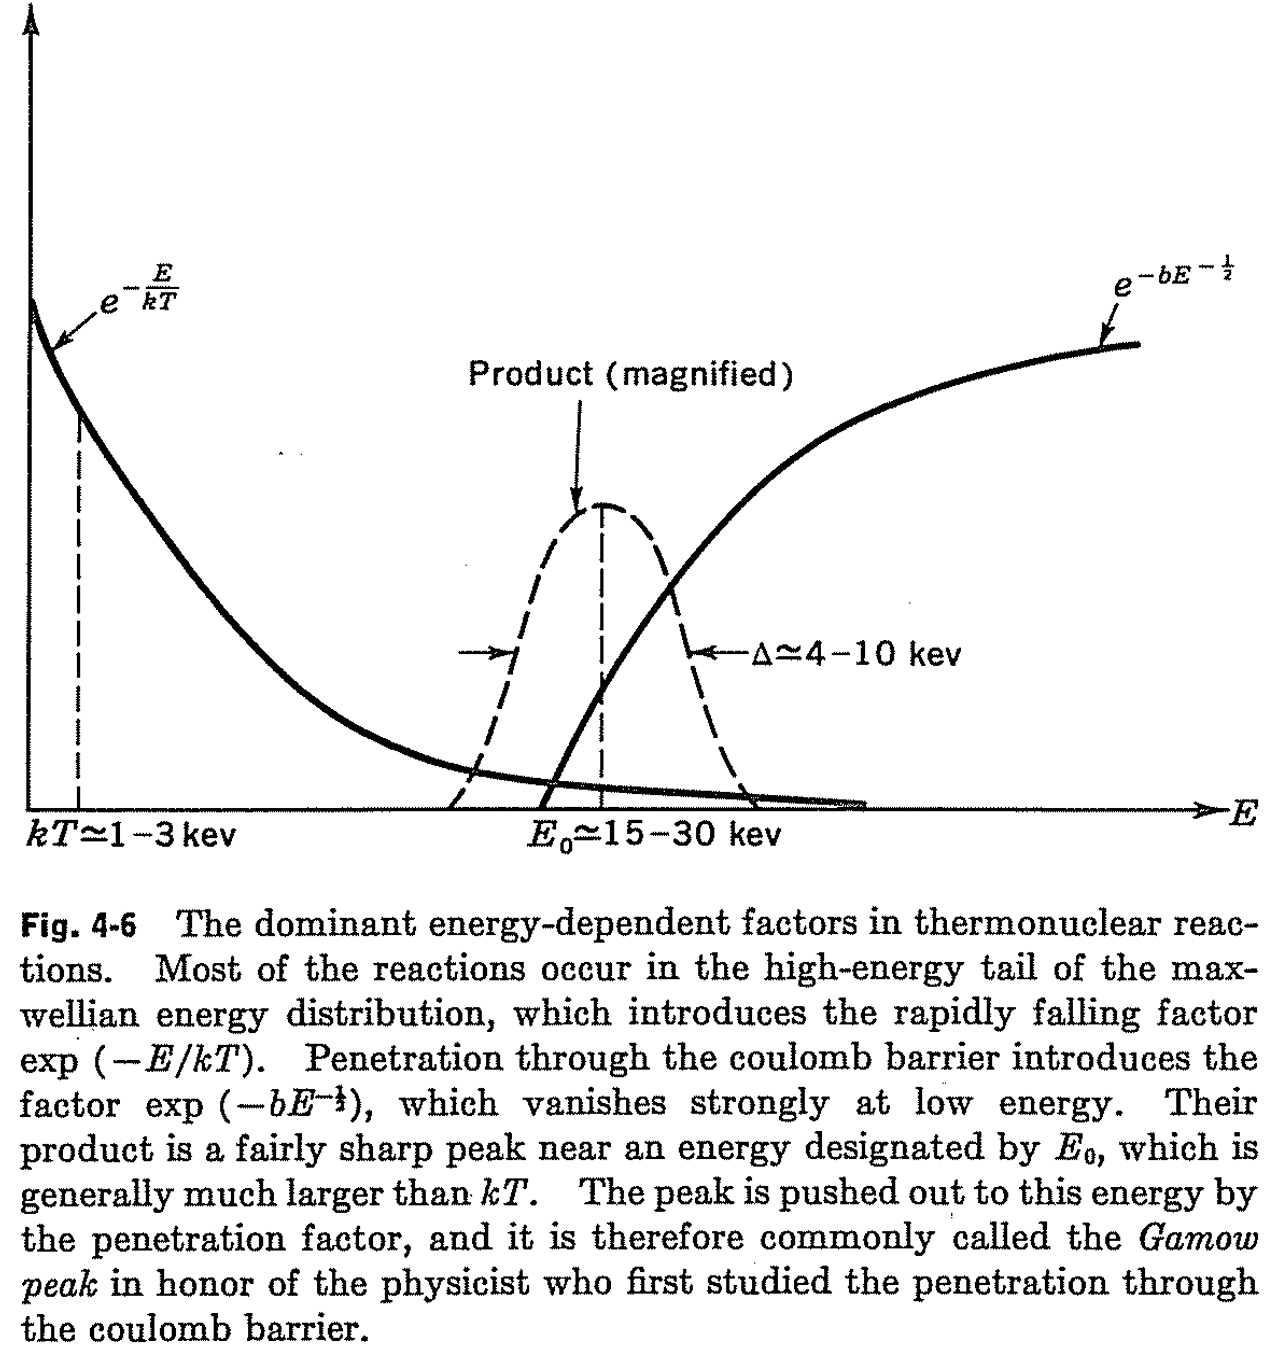
\includegraphics[trim={0.0cm 0cm 0.0cm 0},clip, keepaspectratio,width=0.8\textwidth]{GamowPeak}\label{fig:GamowPeak}
	\end{figure}
    \begin{itemize}
                    \item Probability crossing Coulomb barrier: $P_0(E)=\exp{-\frac{2\pi Z_1Z_2e^2}{\hbar v}}$
                    \item geometrical crosssection $\pi\lambda^2\propto p^{-2}\propto\invers{E}$
                    \item definendo il fattore astrofisico $S(E)$: $\sigma(E)=\frac{S(E)}{E}\exp{-\frac{2\pi Z_1Z_2e^2}{\hbar v}}$
                    \item G-peak: max $\exp{-\frac{E}{KT}-\frac{b}{E^{-\frac{1}{2}}}}$ is $E_0=(\frac{bKT}{2})^{\frac{2}{3}}$
        \end{itemize}
        \end{column}
    \end{columns}
    \begin{itemize}
        \end{itemize}
\end{frame}

\subsection{Radiation}

\begin{frame}{Radiation}
    \begin{columns}[T]
        \begin{column}{0.6\textwidth}
    \begin{align*}
        &F=\int I\cos{\theta}d\Omega=2\pi\int_{-1}^1I\mu d\mu\si{\erg\per\second\per\square\cm}\tag{Tot z-Flux}\\
        &\TDy{s}{I}=0, I=\frac{j}{\kappa}=\frac{c}{4\pi}aT^4=\frac{\sigma}{\pi}T^4\tag{LTE}\\
        &U=\frac{2\pi}{c}\int_{-1}^1I\,d\mu=\frac{4\pi}{c}I\tag{LTE}\\
        &\mu\PDy{r}{I_{\nu}}+[\frac{(1-\mu^2)}{r}\PDy{\mu}{I_{\nu}}]=j_{\nu}-\kappa_{\nu}I_{\nu}\tag{Rad.Transf}\\
        &\TDof{s}=\mu\PDof{r}+\frac{1-\mu^2}{r}\PDof{\mu}\\
        &\mu\TDy{x}{I_{\nu}(\mu,x)}=\j_{\nu}(x)-\kappa_{\nu}(x)I_{\nu}(\mu,x)\tag{plane p.}\\
        &\mu\TDy{\tau_{\nu}}{I_{\nu}(\mu,\tau_{\nu})}=I_{\nu}(\mu,\tau_{\nu})-S_{\nu}(\tau_{\nu})\\
        &\TDof{\tau}[\exp{-\frac{\tau}{\mu}}I]=-\exp{-\frac{\tau}{\mu}}\frac{S}{\mu}\tag{Int.factor}\\
        &\Rightarrow I(\tau,\mu)=\exp{-\frac{(\tau_0-\tau)}{\mu}}I(\tau_o,\mu)+\int_{\tau}^{\tau_0}\exp{-\frac{(t-\tau)}{\mu}}\frac{S(t)}{\mu}\,dt\\
        &\vec{F}_{\nu}=\int d\Omega I(\vec{x},t;\hat{n},\nu)\hat{n}=(\int I_{\nu}n_xd\Omega,\int I_{\nu}n_yd\Omega,\int I_{\nu}n_zd\Omega)\\
        &n_x=\sqrt{1-\mu^2}\cos{\phi},n_y=\sqrt{1-\mu^2}\sin{\phi},n_z=\mu
    \end{align*}
            
        \end{column}
        \begin{column}{0.4\textwidth}
            \begin{itemize}
                \item Photon momentum: $\frac{E}{c}$
                \item Mass emission coeff. $j(\theta)$ (\si{\erg\per\second\per\gram}): Put into $\theta$ - $dI=j(\theta)\rho\,ds$
                \item Absorption coeff $\kappa$: Taken out of $\theta$ - $dI=-\kappa\rho I(\theta)\,ds$
                \item Optical depth: $d\tau_{\nu}=-\kappa_{\nu}\rho\,dz$, $\tau_{\nu}(z)=\tau_{\nu,0}-\int_{z_0}^z\kappa_{\nu}\rho\,dz$ if $z_0$ is true surf. $\tau_{\nu,0}=0$
                \item BlackBody: $B_{\nu}$: BlackBody Intensity, $\pi B_{\nu}$: BlackBody Flux
                \item First Moment - Eddington Flux: $H_{\nu}=\frac{1}{4\pi}\int I_{\nu}\cos{\theta}\,d\Omega=\frac{1}{2}\int_{-1}^1I_{\nu}\mu\,d\mu=\frac{F_{\nu}}{4}$
                \item Mean intensity(0-th moment of rad-field over angles): $J_{\nu}=\frac{1}{4\pi}\int\,d\Omega I(\vec{x},t;\hat{n},\nu)$. PP: $J_{\nu}=\frac{1}{2}\int_{-1}^1I(z,t;\mu,\nu)d\mu$.
                \end{itemize}
        \end{column}
    \end{columns}
    
\end{frame}

\begin{frame}{BlackBody}
    
\end{frame}

\begin{frame}{Radiation Transfer in far interior and Diffusion analogy}
    \begin{columns}[T]
        \begin{column}{0.5\textwidth}
            \begin{align*}
                &I_{\nu}^{out}(\tau_{\nu},\mu)=\int_{\tau_{\nu}}^{\infty}[B_{\nu}(\tau_{\nu})+\TDy{\tau_{\nu}}{B_{\nu}}(t-\tau_{\nu})]\exp{-\frac{(t-\tau_{\nu})}{\mu}}\frac{dt}{\mu}\\
                    &=\int_0^{\infty}[B_{\nu}(\tau_{\nu})+\TDy{\tau_{\nu}}{B_{\nu}}\mu u]\exp{-u}\,du\\
                    &\Rightarrow I(\tau,\mu\geq0)=B(\tau)+\mu(\PDy{\tau}{B})_{\tau}\\
                    &H_{\nu}=\frac{F_{\nu}}{4}=\frac{1}{2}\int_{-1}^1\mu I_{\nu}\,d\mu=\frac{1}{3}\TDy{\tau_{\nu}}{B_{\nu}}\\
                    &=-\frac{1}{3}\frac{1}{\kappa_{\nu}}\TDy{\tau_{\nu}}{B_{\nu}}=-\frac{1}{3\kappa_{\nu}}\TDy{T}{B_{\nu}}\TDy{x}{T}
            \end{align*}
        \end{column}
        \begin{column}{0.5\textwidth}
            \begin{itemize}
                \item Diffusion approx: $\tau_{\nu}\gg1$
                    \item Solution in far interior:
                        \begin{align*}
                            &J_{\nu}(\tau_{\nu})=B_{\nu}(\tau_{\nu})+\frac{1}{3}(\PtwoDy{\tau_{\nu}}{B_{\nu}})+\ldots\\
                            &H_{\nu}(\tau_{\nu})=\frac{1}{3}\PDy{\tau_{\nu}}{B_{\nu}}+\frac{1}{5}\partial^3\ldots\\
                            &K_{\nu}(\tau_{\nu})=\frac{1}{3}\PDy{\tau_{\nu}}{B_{\nu}}+\frac{1}{5}\PDy{\tau_{\nu}}{B_{\nu}}+\ldots\\
                            &\Rightarrow J_{\nu}=3K_{\nu}=B_{\nu}, H_{\nu}=\frac{1}{3}\PDy{\tau_{\nu}}{B_{\nu}}
                        \end{align*}
            \end{itemize}
        \end{column}
    \end{columns}
    Integrating over freq:
    \begin{align*}
        &F=-\frac{4\pi}{3}[\int_0^{\infty}\chi_{\nu}^{-1}\PDy{\tau_{\nu}{B_{\nu}}}\,d\nu]\TDy{r}{T}\tag{int $H_{\nu}$ over freq.}\\
        &\vec{F}=-K_R\nabla T,K_R=\frac{4\pi}{3\chi_R}\TDy{T}{B}=\frac{4}{3}c\lambda_RaT^3\\
        &\chi_R^{-1}=\frac{\int_0^{\infty}\chi_{\nu}^{-1}\TDy{T}{B_{\nu}}\,d\nu}{\int_0^{\infty}\TDy{T}{B_{\nu}}\,d\nu}
        &\chi=\kappa+\sigma
    \end{align*}
\end{frame}

\subsection{Energies}

\begin{frame}{Q-valore, Mass excess - PP chain}
    \begin{columns}[T]
        \begin{column}{0.5\textwidth}
\begin{itemize}
    \item $m_{atom}(A,Z)=m_{nuc}(A,Z)+Zm_e-B_e(Z)$, $\massexcess{}=(m_{atom}-Am_u)c^2$, $Q_{I\to F}=\sum_Im_Ic^2-\sum_Fm_Fc^2=\sum_I\massexcess{I}-\sum_F\massexcess{F}$, $B(Z,A)=(Zm_p+Nm_n-m_{nuc})c^2$, $m_{nuc}=Zm_p+Nm_n-\Delta m$, $m_uc^2=\SI{931.494}{\mega\ev}$.
    \item $^{17}O+p\to\alpha+^{14}N$:
        \begin{align*}   
        &Q=\massexcess{^{17}O}+\massexcess{^1H}-\massexcess{^{14}N}-\massexcess{\alpha}\\
        &=[\num{-808.81}+\num{7288.97}-\num{2863.42}-\num{2424.92}]\si{\kilo\ev}\\
        &=m_{^{17}O}+m_{1^H}-m_{^{14}N}-m_{\alpha}
    \end{align*}
    \item $p+p\to^2H\APelectron+\Pnue$:
        \begin{align*}
            &Q=(2*m_{^1H}-m_{^2H})c^2\\
            &=2*\massexcess{^1H}-\massexcess{^2H}\tag{contains $2m_ec^2$}\\
            &=2*\SI{7288.97}{\kilo\ev}-\SI{13135.72}{\kilo\ev}=\SI{1442.22}{\kilo\ev}\\
            &Q=[2\overbrace{(m_p+m_e)}^{m_{^1H}}-(m_d+m_e)]c^2\\
            &=[(m_p+m_p-m_d-m_e)+2m_e]c^2
        \end{align*}
    \end{itemize}
        \end{column}
        \begin{column}{0.5\textwidth}
            \begin{figure}[!ht]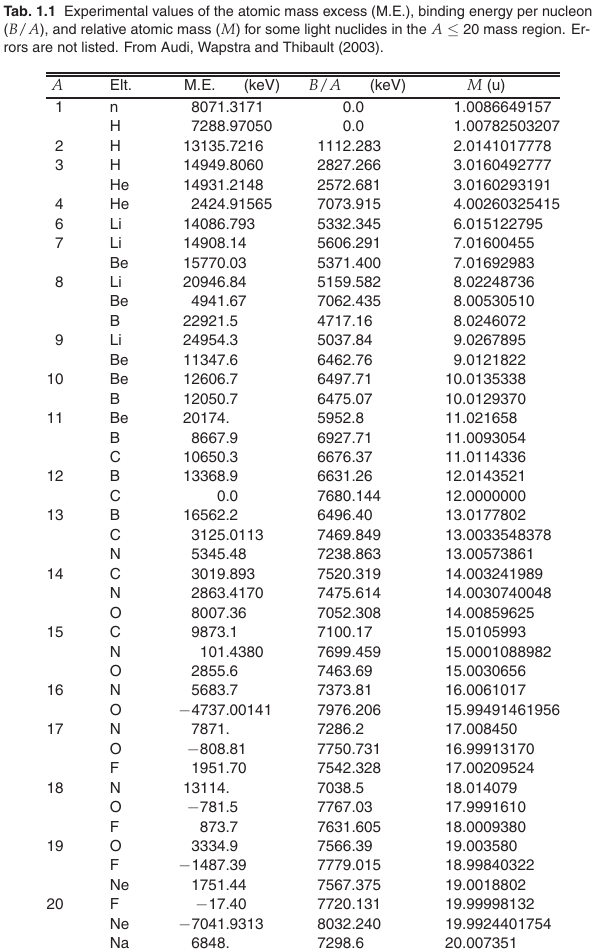
\includegraphics[trim={0.0cm 0cm 0.0cm 0},clip, keepaspectratio,height=0.9\textheight]{mass-excess}\label{fig:mass-excess}
			\end{figure}
        \end{column}
    \end{columns} 
\end{frame}

\begin{frame}{Binding Energies}
    \begin{columns}[T]
        \begin{column}{0.5\textwidth}
            \begin{align*}
                &m_uc^2=\SI{931.494}{\mega\ev}\\
                &m_{nuc}=Zm_p+Nm_n-\Delta m\\
                &B(Z,A)=(Zm_p+Nm_n-m_{nuc})c^2\\
                &2d\to\alpha:\\
                &\frac{B(d)}{A}=\SI{1.112}{\mega\ev},\frac{B(\alpha)}{A}=\SI{7.074}{\mega\ev}\\
                &Q=\SI{28.296}{\mega\ev}-\SI{2.224}{\mega\ev}-\SI{2.224}{\mega\ev}\\
                &=\SI{23.85}{\mega\ev}\tag{En. release}
            \end{align*}
        \end{column}
        \begin{column}{0.5\textwidth}
            \begin{figure}[!ht]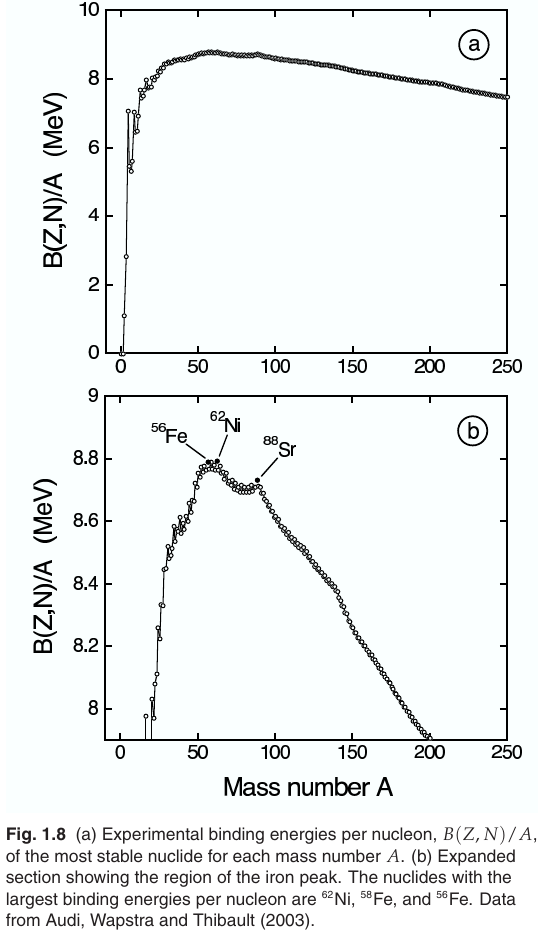
\includegraphics[trim={0.0cm 0cm 0.0cm 0},clip, keepaspectratio,height=0.9\textheight]{binding-energy}\label{fig:binding-energy}
			\end{figure}
        \end{column}
    \end{columns}
\end{frame}

\subsection{EOS}

\begin{frame}{Gas perfetto, elettroni degeneri}
    \begin{columns}[T]
        \begin{column}{0.5\textwidth}
            \begin{align*}
                &P_g=P_I+P_e=\frac{\rho}{\mu}RT=nKT\\
                &\frac{d\rho}{\rho}=\frac{dP}{P}-\frac{dT}{T}+\frac{d\mu}{\mu}\\
                &\mu=\frac{1}{\exv{n_H}X+\exv{n_{He}}+\exv{n_Z}Z}\tag{massa media free part}\\
                &\invers{\mu}=\sum_iX_i\frac{1+f_i}{A_i}\\
                &\mu_0=\frac{1}{X+\frac{Y}{4}+\frac{Z}{\exv{A}}}\\
                &\mu_e\approx(\frac{1}{1}X+\frac{2}{4}Y)^{-1}=\frac{2}{1+X}\tag{full ion.}\\
                &u=\frac{1}{\rho}\sum\int f^{(0)}(p_i)\frac{p_i^2}{2m_i}d^3p_i\tag{internal ener. per unit mass}\\
                &=\frac{3}{2}\frac{P}{\rho}=\frac{3}{2}\frac{RT}{\mu}
            \end{align*}
        \end{column}
        \begin{column}{0.5\textwidth}
            Degenerazione elettronica
            \begin{align*}
                &f(\vec{p})=\left\{\begin{array}{l}
                        \frac{8\pi p^2}{h^3}: p\leq p_F\\
                        0: p>p_F\\
                \end{array}\\\right.
                    &n_edV=dV\int_0^{p_F}\frac{8\pi}{h^3}p^2dp=\frac{8\pi}{3h^3}p_F^3\,dV\\
                    &\Rightarrow p_F\propto n_e^{\frac{1}{3}}, E_F=\frac{p_F^2}{2m_e}\propto n_e^{\frac{2}{3}}\\
                    &P_e=\int \frac{d\Omega_s}{4\pi}\int_0^{\infty}f(p)v(p)p\cos^2{\theta}dp\\
                    &=\frac{8\pi}{3h^3}\int_0^{p_F}p^3v(p)dp=\frac{8\pi c}{3h^3}\int_0^{p_F}\frac{\frac{p}{m_ec}dp}{\sqrt{1+\frac{p^2}{m_e^2c}}}\\
                    &=\frac{\pi m_e^4c^5}{3h^3}f(x)=\left\{\begin{array}{l}
                            x\ll1: \frac{8\pi m_e^4c^5}{15h^3}x^5=\frac{2}{3}U_e\\
                            x\gg1: \frac{2\pi m_e^4c^5}{3h^3}x^4=\frac{1}{3}U_e\\
                    \end{array}\right.
            \end{align*}
        \end{column}
    \end{columns}
    \begin{columns}[T]
        \begin{column}{0.55\textwidth}
    \begin{align*}
                    &U_e=\int_0^{p_F}f(p)E(p)d^3p=\frac{8\pi}{h^3}\int_0^{p_F}E(p)p^2dp=\frac{\pi m_e^4c^5}{3h^3}g(x)\\
                    &x=\frac{p_F}{m_ec}, x\ll1:\left\{\begin{array}{l}
                            f(x)\approx \frac{8}{5}x^5\\
                            g(x)\approx \frac{12}{5}x^5\\
                    \end{array}\right.,\  x\gg1:\left\{\begin{array}{l}
                            f(x)\approx 2x^4\\
                            g(x)\approx 6x^4\\
                    \end{array}\right.
    \end{align*}
        \end{column}
        \begin{column}{0.45\textwidth}
            \begin{align*}
            &P_e= \left\{\begin{array}{l}
                    x\ll1: \frac{1}{20}(\frac{3}{\pi})^{\frac{2}{3}}\frac{h^2}{m_e}n_e^{\frac{5}{3}}\\
                            x\gg1: (\frac{3}{\pi})^{\frac{1}{3}}\frac{hc}{8}n_e^{\frac{4}{3}}\\
                    \end{array}\right.\\
            &\left\{\begin{array}{l}
                            \frac{1}{20}(\frac{3}{\pi})^{\frac{2}{3}}\frac{h^2}{m_em_u^{\frac{5}{3}}}(\frac{\rho}{\mu_e})^{\frac{5}{3}}=\num{1.0036e13}(\frac{\rho}{\mu_e})^{\frac{5}{3}}\si{\cgs}\\
                            (\frac{3}{\pi})^{\frac{1}{3}}\frac{hc}{8m_u^{\frac{4}{3}}}(\frac{\rho}{\mu_e})^{\frac{4}{3}}=\num{1.2435e15}(\frac{\rho}{\mu_e})^{\frac{4}{3}}\si{\cgs{}}\\
                    \end{array}\right.
                \end{align*}
        \end{column}
    \end{columns}
    
\end{frame}

\subsection{CrossSection}

\begin{frame}{Nuclear elastic scattering: \schr{} eq., partial waves}
    \begin{columns}[T]
        \begin{column}{0.55\textwidth}
            \begin{align*}
                &\psi=f(r)Y_l^m(\theta,\phi), L=\vecp{r}{p}=\frac{\hbar}{i}\vecp{r}{\nabla}\\
                &-\frac{\hbar^2}{2\mu}\nabla^2\psi+V(r)\psi=E\psi\\
                &-\frac{\hbar^2}{2\mu}=-\frac{\hbar^2}{2\mu}(\PtwoDof{r}+\frac{2}{r}\PDof{r})+\frac{L^2}{2\mu r^2}=\frac{p_r^2}{2\mu}+\frac{L^2}{2\mu r^2}\\
                &-\frac{\hbar^2}{2\mu}\TtwoDy{r}{\chi_l}+[\frac{l(l+1)\hbar^2}{2\mu r^2}+V(r)-E]\chi_l=0\tag{$f_l=\frac{\chi_l(r)}{r}$}\\
                &\psi(\vec{r})=N[\exp{i\scap{k}{r}}+f(\theta)\frac{\exp{ikr}}{r}]\tag{beam+target, $r\to\infty$}\\
                &\exp{i\scap{k}{r}}\to\exp{ikz}:u_l^{f.p.}=(kr)j_l(kr)\tag{free p.: Sol $j_l(kr)$ sph. Bessel}\\
                &\xrightarrow{\to\infty}\sin{(kr-\frac{l\pi}{2})},u_{l=0}^{f.p.}=\sin{(kr)}\\
                &\psi_T^{f.p.}=\exp{ikz}=\sum_{l=0}^{\infty}\underbrace{(2l+1)i^l}_{c_l}j_l(kr)P_l(\cos{\theta})\\
                &\xrightarrow{\to\infty}\frac{1}{2kr}\sum_{l=0}^{\infty}(2l+1)i^{l+1}[\exp{-i(kr-\frac{l\pi}{2})}-\exp{i(kr-\frac{l\pi}{2})}]P_l(\cos{\theta})\\
                &u_l=\sin{(kr-\frac{l\pi}{2}+\delta_l)}\tag{$r\to\infty$: $V=0$ same eq.}\\
                &\psi_T=\exp{ikz}+f(\theta)\frac{\exp{ikr}}{kr}\\
                &\xrightarrow{r\to\infty}\sum_{l=0}^{\infty}(2l+1)i^l\exp{i\delta_l}\frac{\sin{(kr-\frac{l\pi}{2}+\delta_l)}}{kr}P_l(\cos{\theta})\\
                &=\frac{1}{2kr}\sum_l^{\infty}(2l+1)i^{l+1}[\exp{-i(kr-\frac{l\pi}{2})}-\exp{2i\delta_l}\exp{i(kr-\frac{l\pi}{2})}]P_l(\cos{\theta})
            \end{align*}
        \end{column}
        \begin{column}{0.45\textwidth} 
            \begin{figure}[!ht]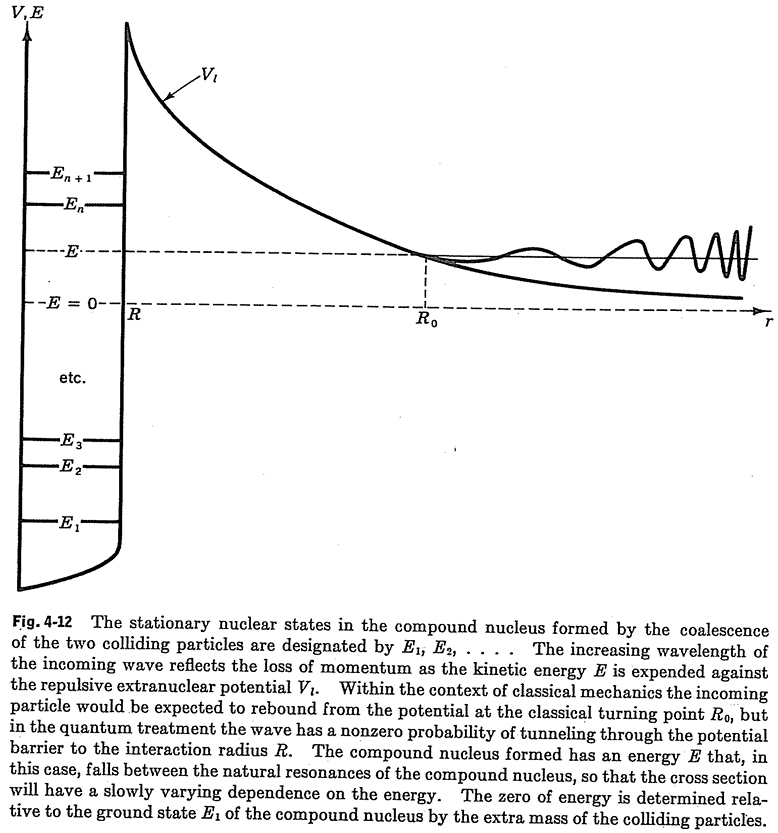
\includegraphics[trim={0.0cm 0cm 0.0cm 0},clip, keepaspectratio,width=0.9\textwidth]{nuclear-potential}\label{fig:nuclear-potential}
			\end{figure}
            \begin{align*}
                &R\approx1.4(A_1^{\frac{1}{3}}+A_2^{\frac{1}{3}})\SI{e-13}{\cm}\\
                &P=\psi^*\psi,j=vP\tag{particle-den, current-d.}\\
                &j_b=N^2v_b, j_s=v_sN^2|f(\theta)|^2 \frac{1}{r^2},dF=r^2d\Omega\\
                &\frac{N_e^{d\Omega}}{t}=\TDy{\sigma}{\Omega}\frac{N_b/t}{A}N_t\,d\Omega\tag{emitted}\\
                &\TDy{\sigma}{\Omega}=\frac{j_{et}\,dF}{j_b\,d\Omega}=\frac{j_sr^2}{j_b}=|f(\theta)|^2,j_{et}=\frac{N_{et}^{d\Omega}}{dF}
            \end{align*}
        \end{column}
    \end{columns}
\end{frame}

\begin{frame}{Elastic Scattering CrossSection}
    \begin{columns}[T]
        \begin{column}{0.7\textwidth}
            \begin{align*}
                &f(\theta)\frac{\exp{ikr}}{kr}=\psi_T-\psi_T^{f.p.}=\frac{1}{2kr}\sum_l(2l+1)i^{l+1}[\exp{i(kr-\frac{l\pi}{2})}(1-\exp{2i\delta_l})]P_l(\cos{\theta})\\
                &\exp{i \frac{\pi l}{2}}=\cos{\frac{\pi l}{2}}+i\sin{\frac{\pi l}{2}}=i^l, \exp{i\delta}\sin{\delta}=\frac{i}{2}(1-\exp{2i\delta}):\\
                &f(\theta)=\frac{1}{k}\sum_l(2l+1)\exp{i\delta_l}\sin{\delta_l}P_l(\cos{\theta})\\
                &(\TDy{\Omega}{\sigma})_{el}=f^*(\theta)f^*(\theta)=\frac{1}{k^2}|\sum_l(2l+1)\sin{\delta_l}P_l(\cos{\theta})|^2\\
                &\int_{d\Omega}P_l(\cos{\theta}P_{l'}(\cos{\theta}))\,d\Omega=\frac{4\pi}{2l+1}\delta_{ll'}:\\
                &\sigma_{el}=\sum_l\sigma_{el,l}=\sum_l \frac{\pi}{k^2}(2l+1)|1-\exp{2i\delta_l}|^2=\frac{4\pi}{k^2}(2l+1)\sin^2{\delta_l}
            \end{align*}
        \end{column}
        \begin{column}{0.3\textwidth}
        \end{column}
    \end{columns}
    \begin{columns}[T]
        \begin{column}{0.6\textwidth}
            \begin{align*}
                &(\TDy{\Omega}{\sigma})_{el,0}=\frac{1}{k^2}\sin^2{\delta_0},\sigma_{el,0}=\frac{4\pi}{k^2}\sin^2{\delta_0}\\
                &\delta_l\to\delta_l+\sigma_l:\tag{charged particles}\\
                &f(\theta)=\frac{i}{2k}\sum_l(2l+1)[1-\exp{2i(\delta_l+\sigma_l)}]P_l(\cos{\theta})\\
                &=\frac{i}{2k}\sum_l(2l+1)(1-\exp{2i\sigma_l})P_l(\cos{\theta})\tag{Rutherford s.}\\
                &+\frac{i}{2k}\sum_l(2l+1)\exp{2i\sigma_l}(1-\exp{2i\delta_l})P_l(\cos{\theta})\tag{N+C}
            \end{align*}
        \end{column}
        \begin{column}{0.4\textwidth}
            \begin{align*}
                &1-\exp{2i(\delta_l+\sigma_l)}\\
                &=(1-\exp{2i\sigma_l})+\exp{2i\sigma_l}(1-\exp{2i\delta_l})
            \end{align*}
        \end{column}
    \end{columns}
    
\end{frame}

\begin{frame}{Reaction CrossSection}
    \begin{columns}[T]
        \begin{column}{0.5\textwidth}
            \begin{align*}
                &\int_{\Omega}j_T\,d\Omega=0\tag{elastic}\\
                &\sigma_{re}=\frac{r^2}{j_b}\int j_T\,d\Omega\tag{non elastic: net current of particles}\\
                &j_b=\frac{\hbar}{2mi}[\exp{-ikz}(\exp{ikz}ik)-\exp{-ikz}(-ik)\exp{ikz}]=\frac{\hbar k}{m}\\
                &j_T=\frac{\hbar}{4mkr^2}[|\sum_l(2l+1)i^{l+1}\exp{\frac{il\pi}{2}}P_l(\cos{\theta})|^2\\
                &-|\sum_l(2l+1)i^{l+1}\exp{2i\delta_l}\exp{\frac{-il\pi}{2}}P_l{\cos{\theta}}|^2]\\
                &\sigma_{re,l}=\frac{\pi}{k^2}(2l+1)(1-|\exp{2i\delta_l}|^2)\geq0\\
                &|\exp{2i\delta_l}|^2=1\tag{If $\delta_l$ real: only elastic-sc}\\
                &\sigma_{el,l}^{max}=\frac{4\pi}{k^2}(2l+1), \sigma_{re,l}=0\tag{max elastic-c.s.}\\
                &\sigma_{re,l}^{max}=\sigma_{el,l}=\frac{\pi}{k^2}(2l+1)\tag{max reaction-c.s.}
            \end{align*}
        \end{column}
        \begin{column}{0.5\textwidth}
            \begin{itemize}
                \item  $\psi_T$ represents elastic scattering w.f.
                    \item $j=\frac{\hbar}{2mi}(\psi^*\TDy{r}{\psi}-\TDy{r}{\psi^*}\psi)$
                \end{itemize}
            \begin{figure}[!ht]
                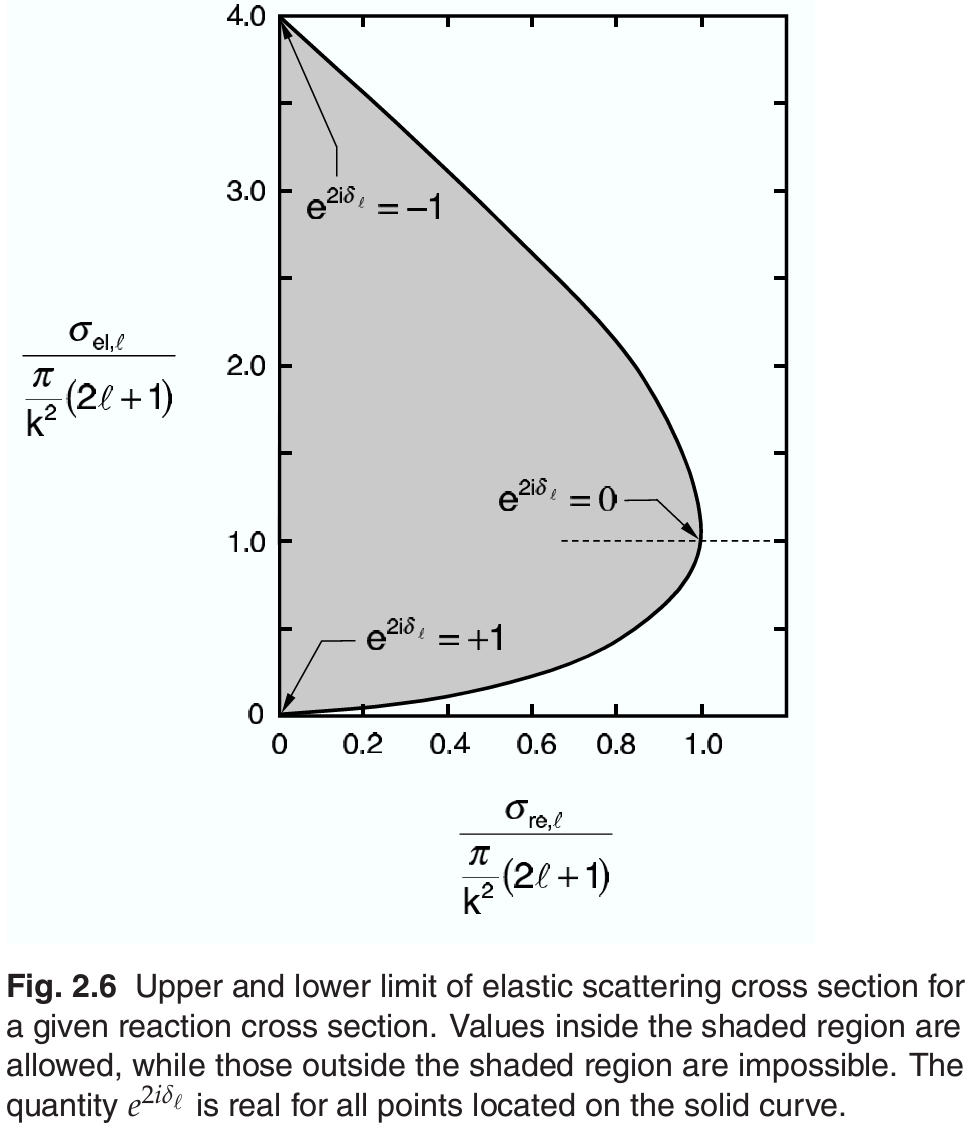
\includegraphics[trim={0.0cm 0cm 0.0cm 0},clip, keepaspectratio,width=0.9\textwidth]{scattering-reaction-cs}\label{fig:scattering-reaction-cs}
			\end{figure}
        \end{column}
    \end{columns}
\end{frame}

\begin{frame}{Transmission prob., phase shift and resonance phenomenon: T defined only in 1D}
    \begin{columns}[T]
        \begin{column}{0.75\textwidth}
        \begin{align*}
            &\TtwoDy{r}{u}+\frac{2m}{\hbar^2}[E-V(r)]u=0: \TtwoDy{r}{u}+\hat{k}u=0\tag{$l=0$, V const}\\
            &u=\alpha\exp{i\hat{k}r}+\beta\exp{-i\hat{k}r}, r<R_0: K^2=\frac{2m}{\hbar^2}(E+V_0), r>R_0: k^2=\frac{2m}{\hbar^2}E\\
            &u_{in}=A'\exp{iKr}B'\exp{-iKr}, u_{in}(0)=0=A'+B'\Rightarrow u_{in}=A\sin{(Kr)}\\
            &u_{out}=C'\exp{ikr}+D'\exp{-ikr}=\tag{$\sin{(x\pm y)}=\sin{x}\cos{y}\pm\cos{x}\sin{y}$}\\
            &C''\sin{(kr)}+D''\cos{(kr)}=C[\sin{(kr)}\cos{\delta_0}+\cos{(kr)}\sin{\delta_0}]=C\sin{(kr+\delta_0)}\\
            &\exp{-i\omega t}\tag{temporal evol: B' propagate negative x, C',D' reflected/moving toward $R_0$}\\
            &j_{tr}=v_{in}|B'|^2, j_{refl}=v_{out}|C'|^2,j_{inc}=v_{out}|D'|^2: T=\frac{j_{tr}}{j_{inc}}=\frac{v_{in}|B'|^2}{v_{out}|D'|^2}=\frac{K|B'|^2}{k|D'|^2}\\
            &\left.\begin{array}{l}&A'\exp{iKR_0}+B'\exp{-iKR_0}=C'\exp{ikR_0}+D'\exp{-ikR_0}\\&\frac{K}{k}(A'\exp{iKR_0}-B'\exp{-iKR_0})=(C'\exp{ikR_0}-D'\exp{-ikR_0})\\
            \end{array}\right\}
            \tag{cont cond}\\
            &\frac{K}{k}(-B'\exp{-iKR_0})=B'\exp{-iKR_0}-2D'\exp{-ikR_0}: \frac{B'}{D'}=2 \frac{\exp{-ikR_0}}{\exp{-iKR_0}}\frac{k}{k+K},A'=0\\
            &T=\frac{K|B'|^2}{k|D'|^2}=4 \frac{kK}{(k+K)^2}=4 \frac{\frac{2m}{\hbar^2}\sqrt{(E+V_0)E}}{[\sqrt{\frac{2m}{\hbar^2}(E+V_0)}+\sqrt{\frac{2m}{\hbar^2}E}]^2}\\
            &\left.\begin{array}{l}&A\sin{(KR_0)}=C\sin{(kR_0+\delta_0)}\\&AK\cos{(KR_0)}=Ck\cos{(kR_0+\delta_0)}\\
            \end{array}\right\}\Rightarrow \frac{1}{K}\tan{(KR_0)}=\frac{1}{k}\tan{(kR_0+\delta_0)}
        \end{align*}
        \end{column}
        \begin{column}{0.25\textwidth}
            \begin{figure}[!ht]
            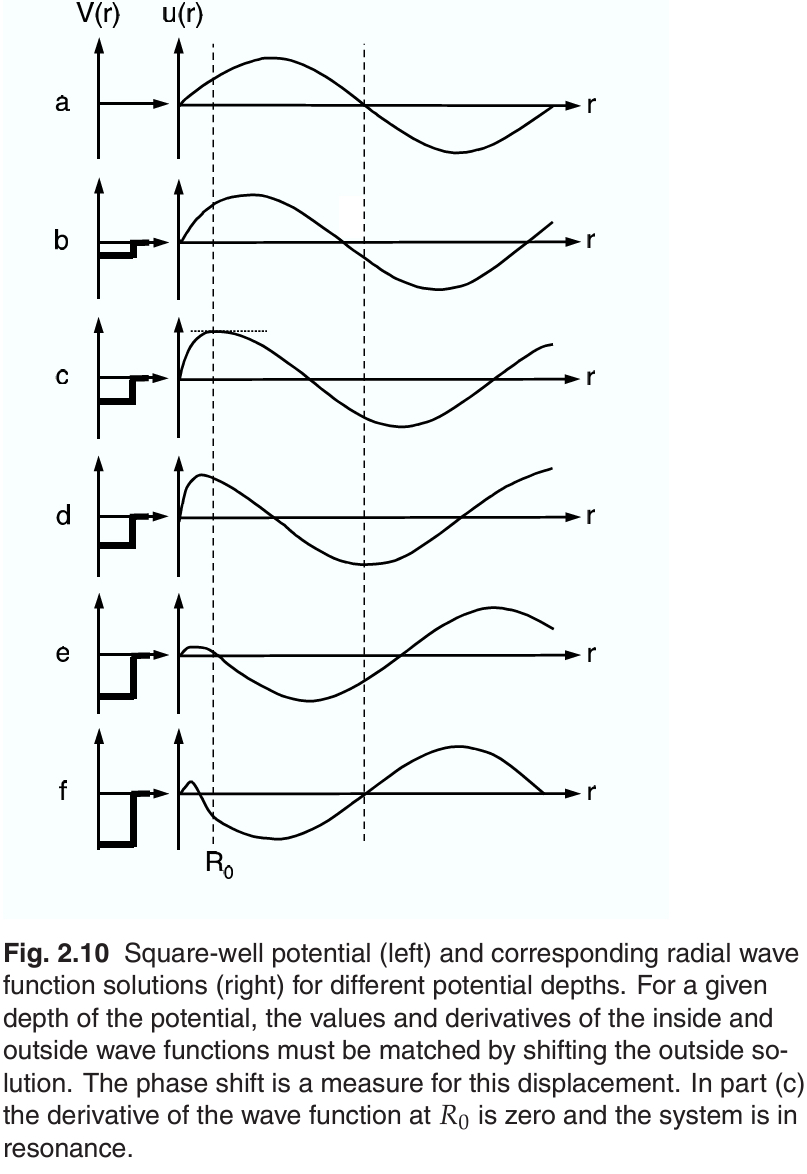
\includegraphics[trim={0.0cm 0cm 0.0cm 0},clip, keepaspectratio,width=0.8\textwidth]{pot-shift}\label{fig:pot-shift}
			\end{figure}
        \end{column}
    \end{columns}
    \begin{align*}
        &\delta_0=-kR_0+\arctan{[\frac{k}{K}\tan{(KR_0)}]}=-\frac{\sqrt{2mE}}{\hbar}R_0+\arctan{[\sqrt{\frac{E}{E*V_0}}\tan{(\frac{\sqrt{2m(E+V_0)}}{\hbar}R_0)}]}\\
        &
    \end{align*}
\end{frame}

\begin{frame}{Resonances}
    Squarin and addin continuity conditions:
    \begin{columns}[T]
        \begin{column}{0.6\textwidth}
        \begin{align*}
            &\frac{|A|^2}{|C|^2}=\frac{k^2}{k^2+[K^2-k^2]\cos^2{(KR_0)}}=\frac{E}{E+V_0\cos^2{(\frac{\sqrt{2m(E+V_0)}}{\hbar}R_0)}}\\
            &\cos^2{KR_0}=0: KR_0=(n+\frac{1}{2})\pi: K=\frac{(n+\frac{1}{2})\pi}{R_0}=\frac{2\pi}{\lambda_{in}}\\
            &\lambda_{in}=\frac{2R_0}{(n+\frac{1}{2})}=\frac{R_0}{(\frac{n}{2}+\frac{1}{4})}\tag{$\lambda_{in}$ wavelength in interior}\\
            &E_n=\frac{\hbar^2}{2m}\frac{\pi^2}{R_0^2}(n+\frac{1}{2})^2-V_0\tag{resonance energy: $\frac{n}{2}+\frac{1}{4}$ wavelength fit into interior}
        \end{align*}
        \begin{columns}[T]
            \begin{column}{0.45\textwidth}
            \begin{figure}[!ht]
            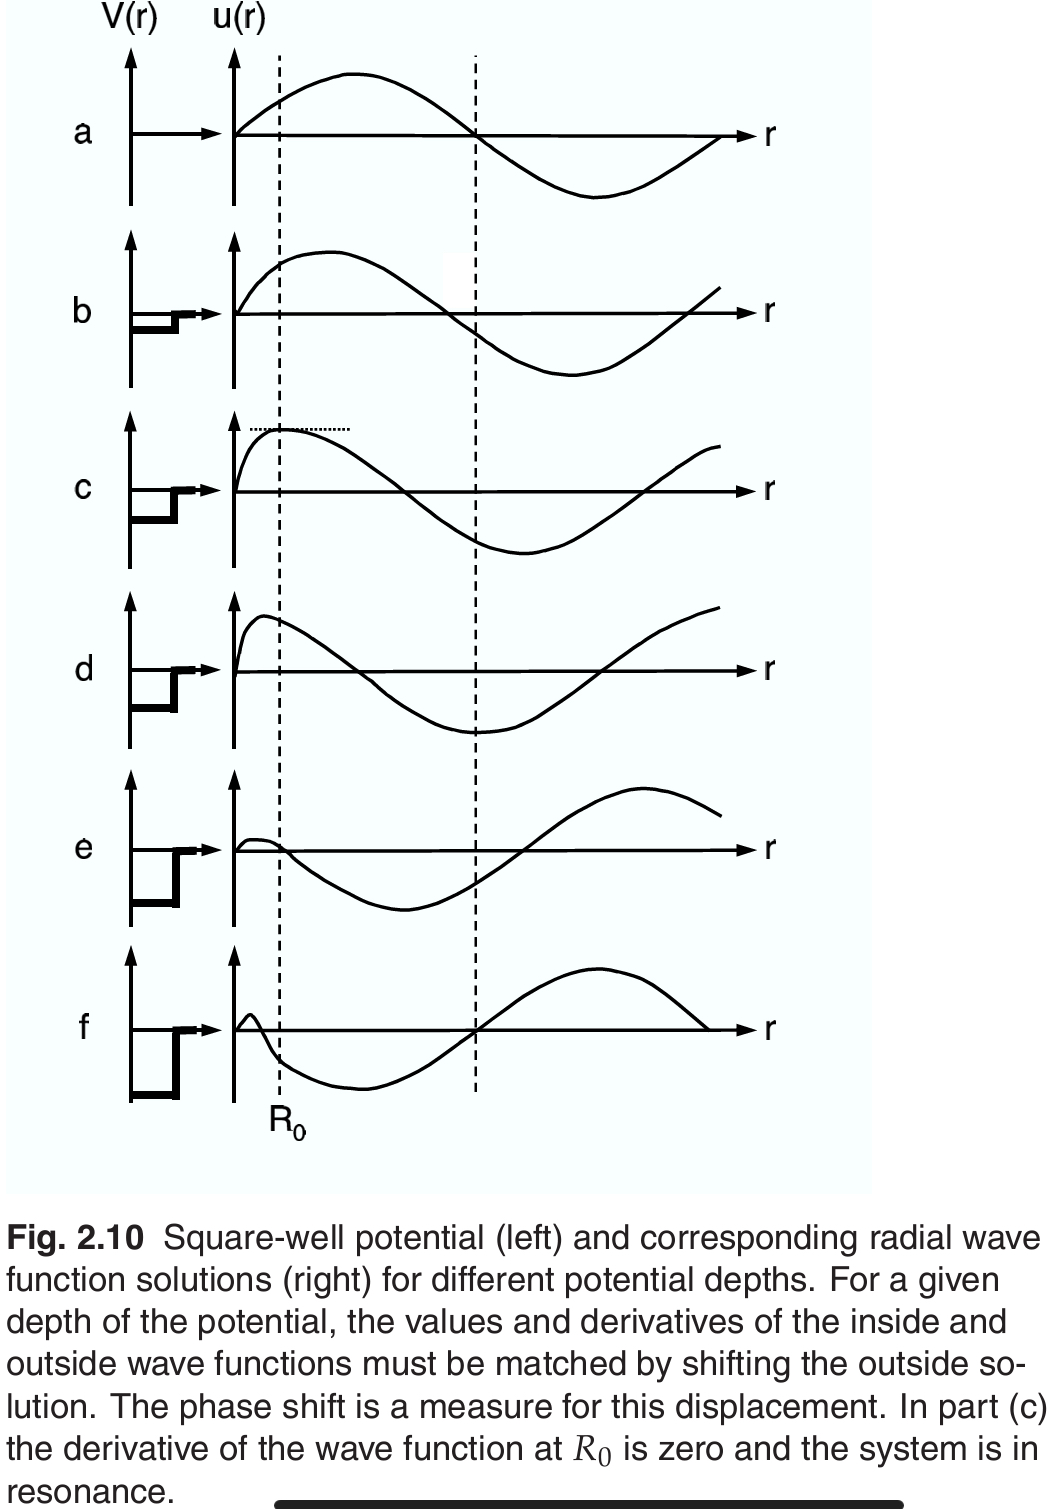
\includegraphics[trim={0.0cm 0cm 0.0cm 0},clip, keepaspectratio,width=0.9\textwidth]{wavefunction-phaseshift}\label{fig:wavefunction-phaseshift}
			\end{figure}
            \end{column}
            \begin{column}{0.55\textwidth}
            \end{column}
        \end{columns}
    \end{column}
        \begin{column}{0.4\textwidth}
            \begin{figure}[!ht]
            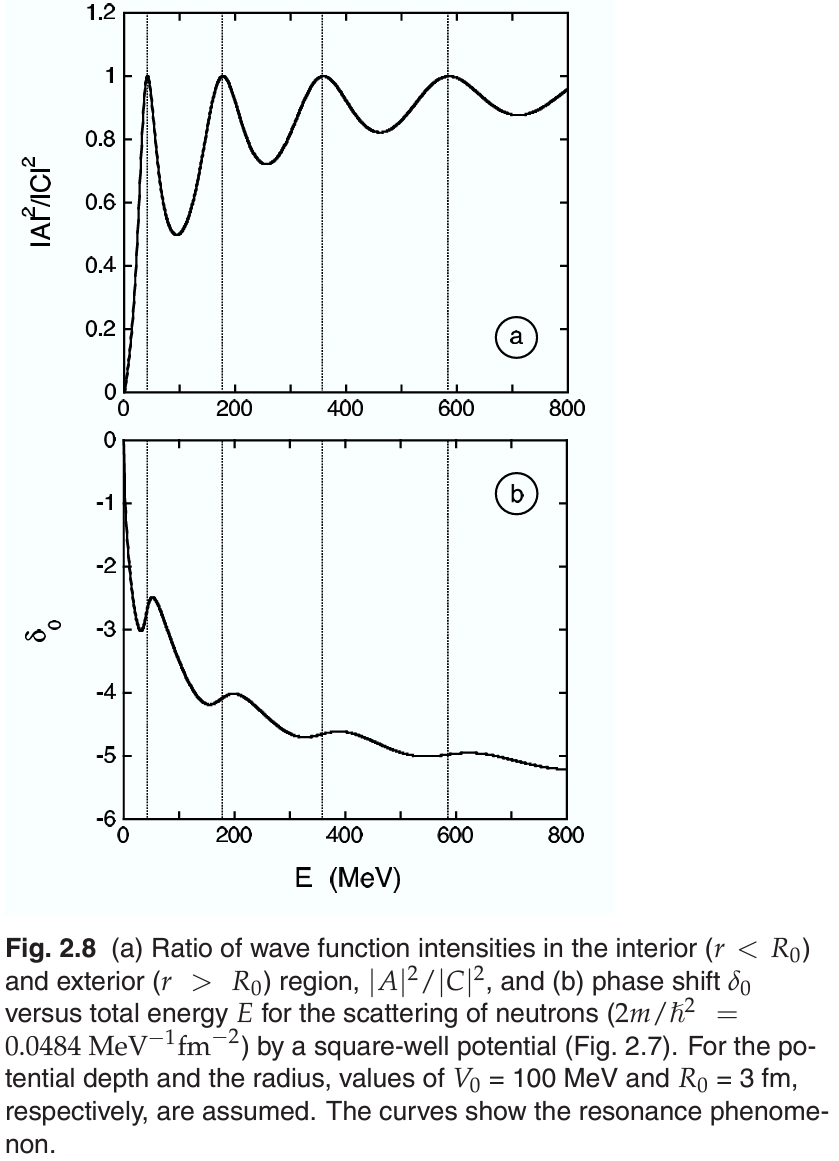
\includegraphics[trim={0.0cm 0cm 0.0cm 0},clip, keepaspectratio,width=0.9\textwidth]{phaseshift-res}\label{fig:phaseshift-res}
			\end{figure}
            At resonance energies $E_i$ prob finding particle inside $r<R_0$ is at maximum; each res shift phase $\delta_0$ by some amount
        \end{column}
    \end{columns}
\end{frame}

\begin{frame}{Resonance in square barrier potential}
                \begin{align*}
                    &u_I=A'\sin{(Kr)},u_{II}=C\exp{-\kappa r}+D\exp{\kappa r}, u_{III}=F'\sin{(kr+\delta_0')},\Delta=R_1-R_0\\
                    &\delta_0=-kR_1+\arctan{[\frac{k}{\kappa}\frac{\sin{(KR_0)}(\exp{-\kappa\Delta}+\exp{\kappa\Delta})+\frac{K}{\kappa}\cos{(KR_0)}(\exp{\kappa\Delta}-\exp{-\kappa\Delta})}{\sin{(KR_0)}(\exp{\kappa\Delta}-\exp{-\kappa\Delta})+\frac{K}{\kappa}\cos{(KR_0)}(\exp{-\kappa\Delta}-\exp{\kappa\Delta})}]}\\
                    &\frac{|F'|^2}{|A'|^2}=\sin^2{KR_0}+(\frac{K}{k})^2\cos^2{(KR_0)}+\sin^2{(KR_0)}\sinh^2{(\kappa\Delta)}[1+(\frac{\kappa}{k})^2]+\cos^2{(KR_0)}\sinh^2{(\kappa\Delta)}[(\frac{K}{\kappa})^2\\
                    &+(\frac{K}{k})^2]+\sin{(KR_0)}\cos{(KR_0)}\sinh{(2\kappa\Delta)}[(\frac{K}{\kappa})+(\frac{K}{\kappa})(\frac{\kappa}{k}^2)]
                \end{align*}
    \begin{columns}[T]
        \begin{column}{0.33\textwidth}
            \begin{figure}[!ht]
            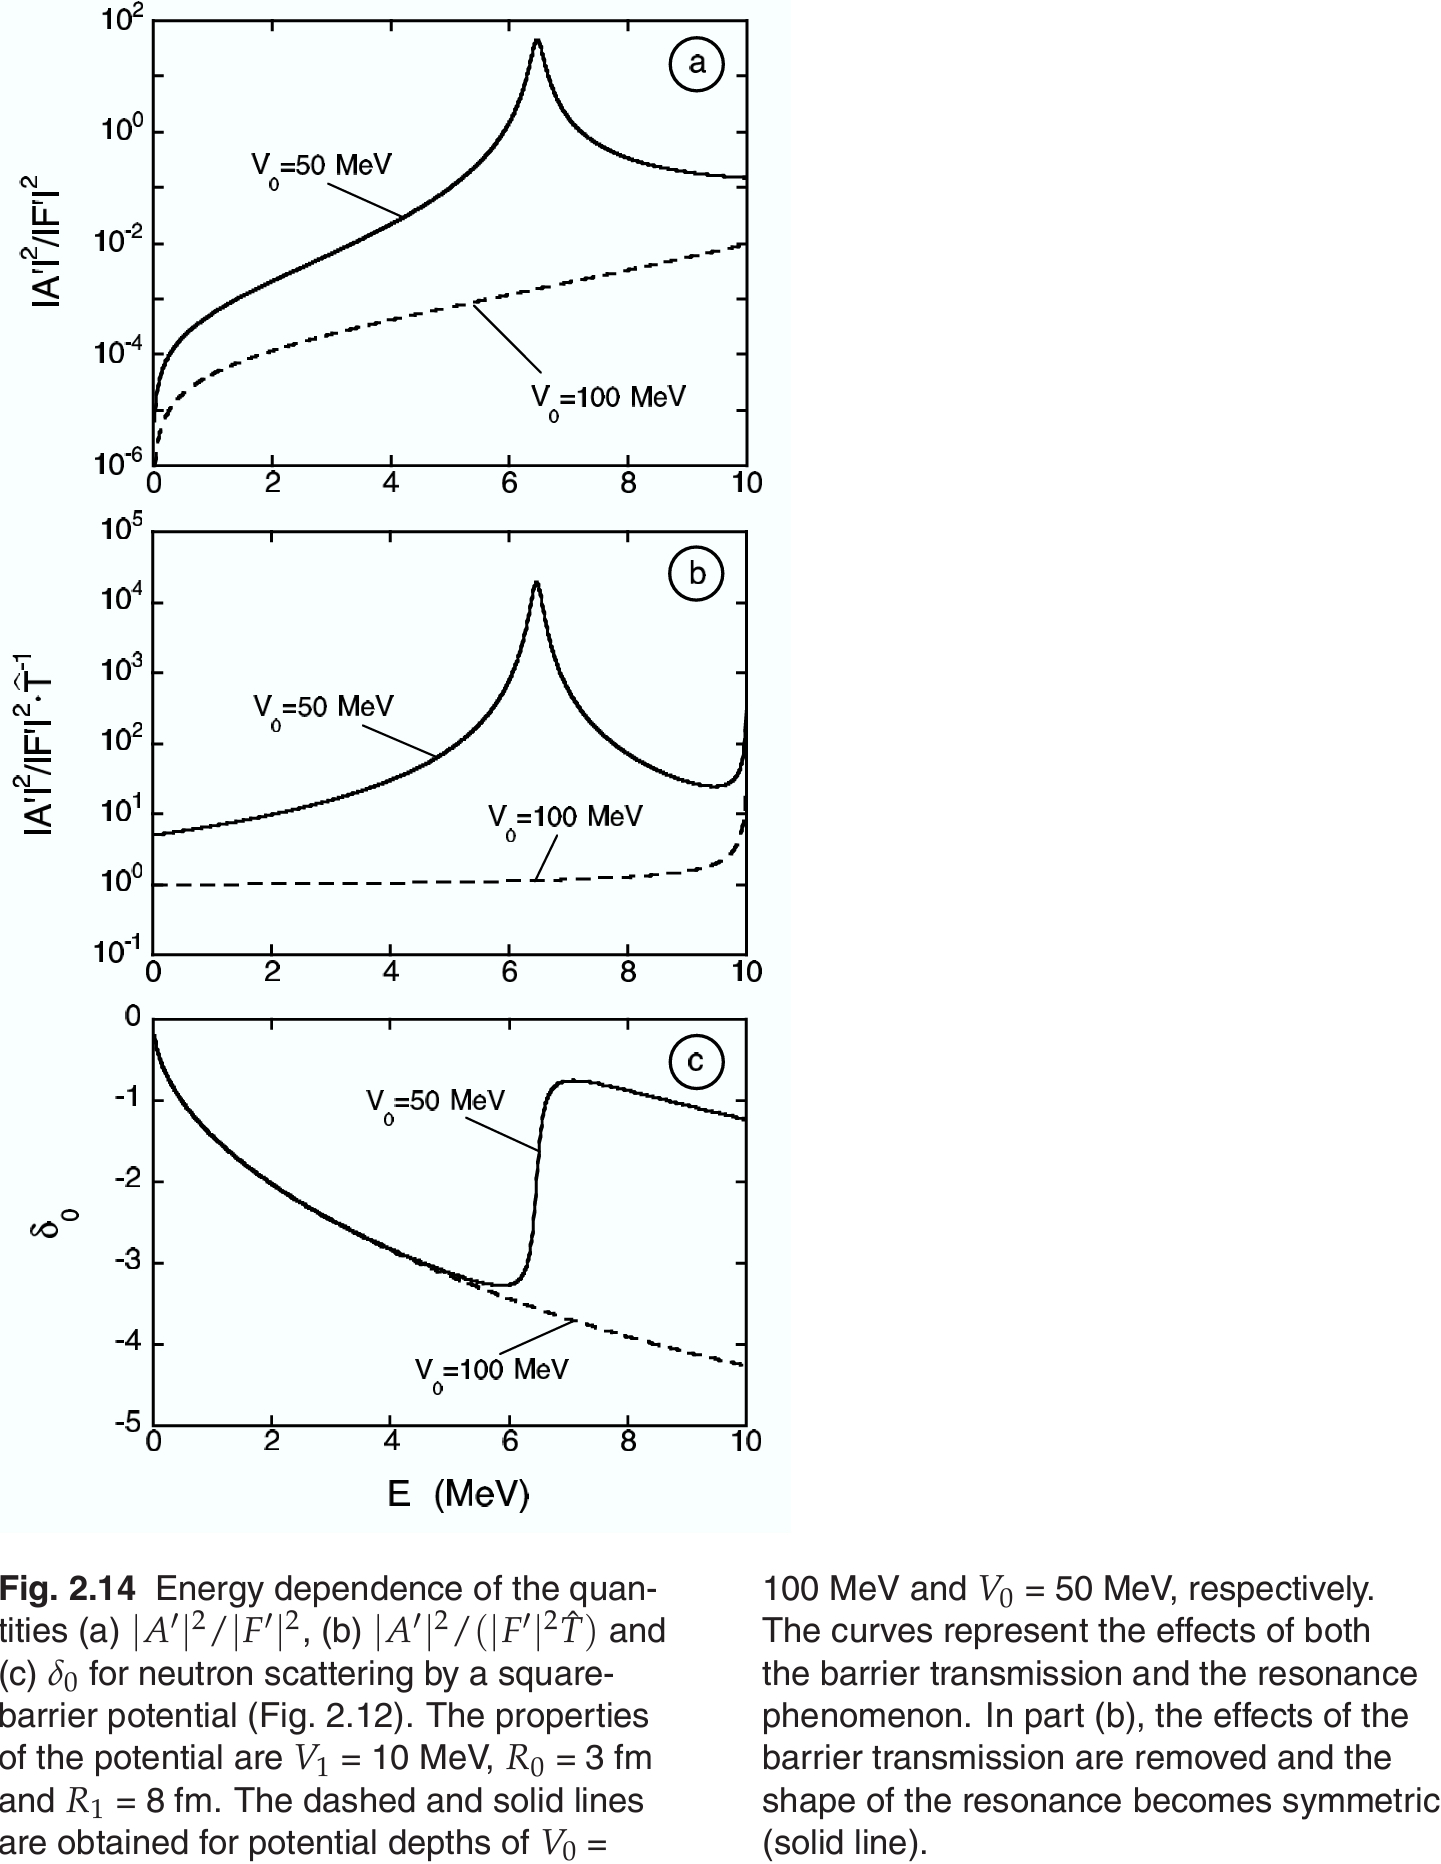
\includegraphics[trim={0.0cm 0cm 0.0cm 0},clip, keepaspectratio,width=0.9\textwidth]{resonance-squarebarrier}\label{fig:resonance-squarebarrier}
			\end{figure}
        \end{column}
        \begin{column}{0.33\textwidth}
            \begin{figure}[!ht]
            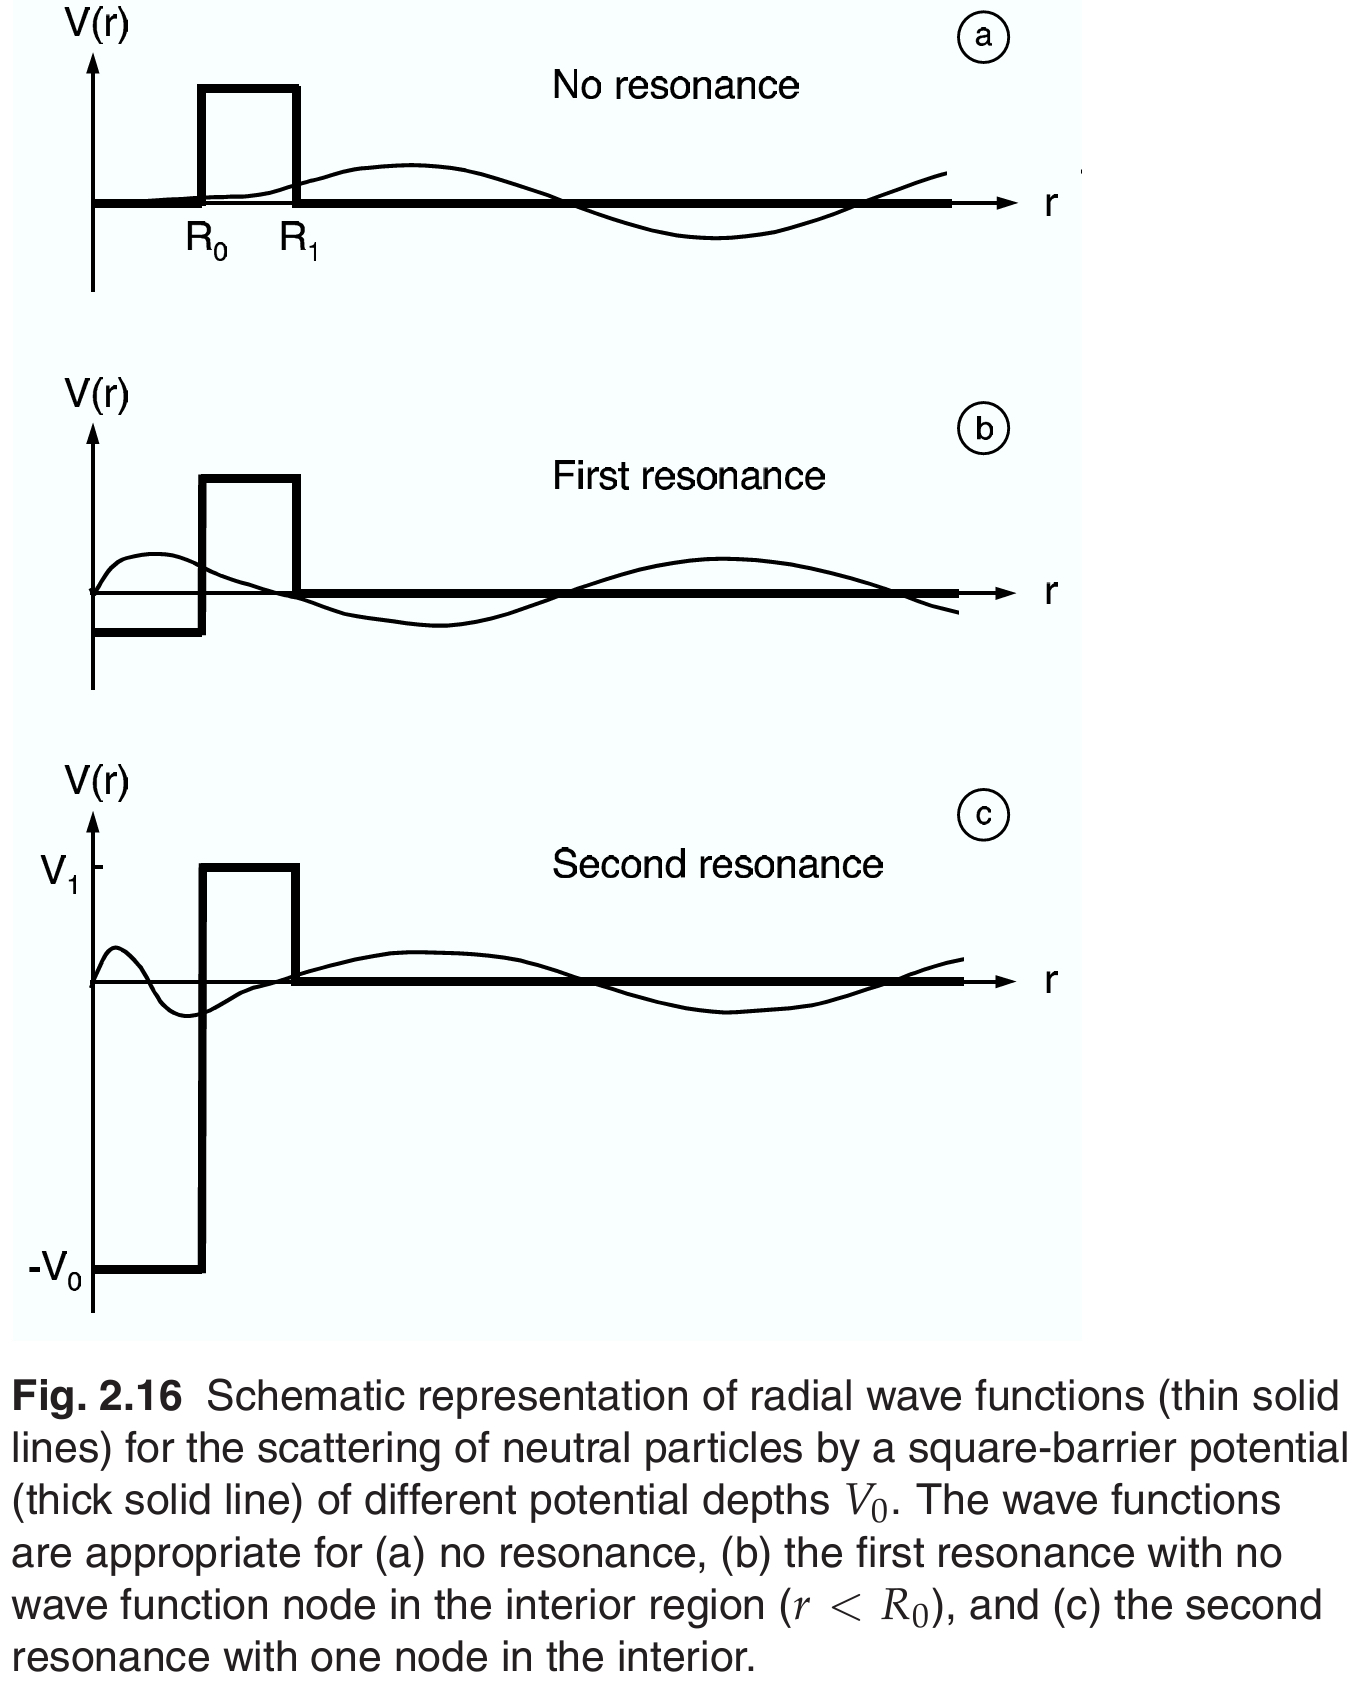
\includegraphics[trim={0.0cm 0cm 0.0cm 0},clip, keepaspectratio,width=0.9\textwidth]{wavefunction-resonance-barrier}\label{fig:wavefunction-resonance-barrier}
			\end{figure}
        \end{column}
        \begin{column}{0.33\textwidth}
            \begin{figure}[!ht]
            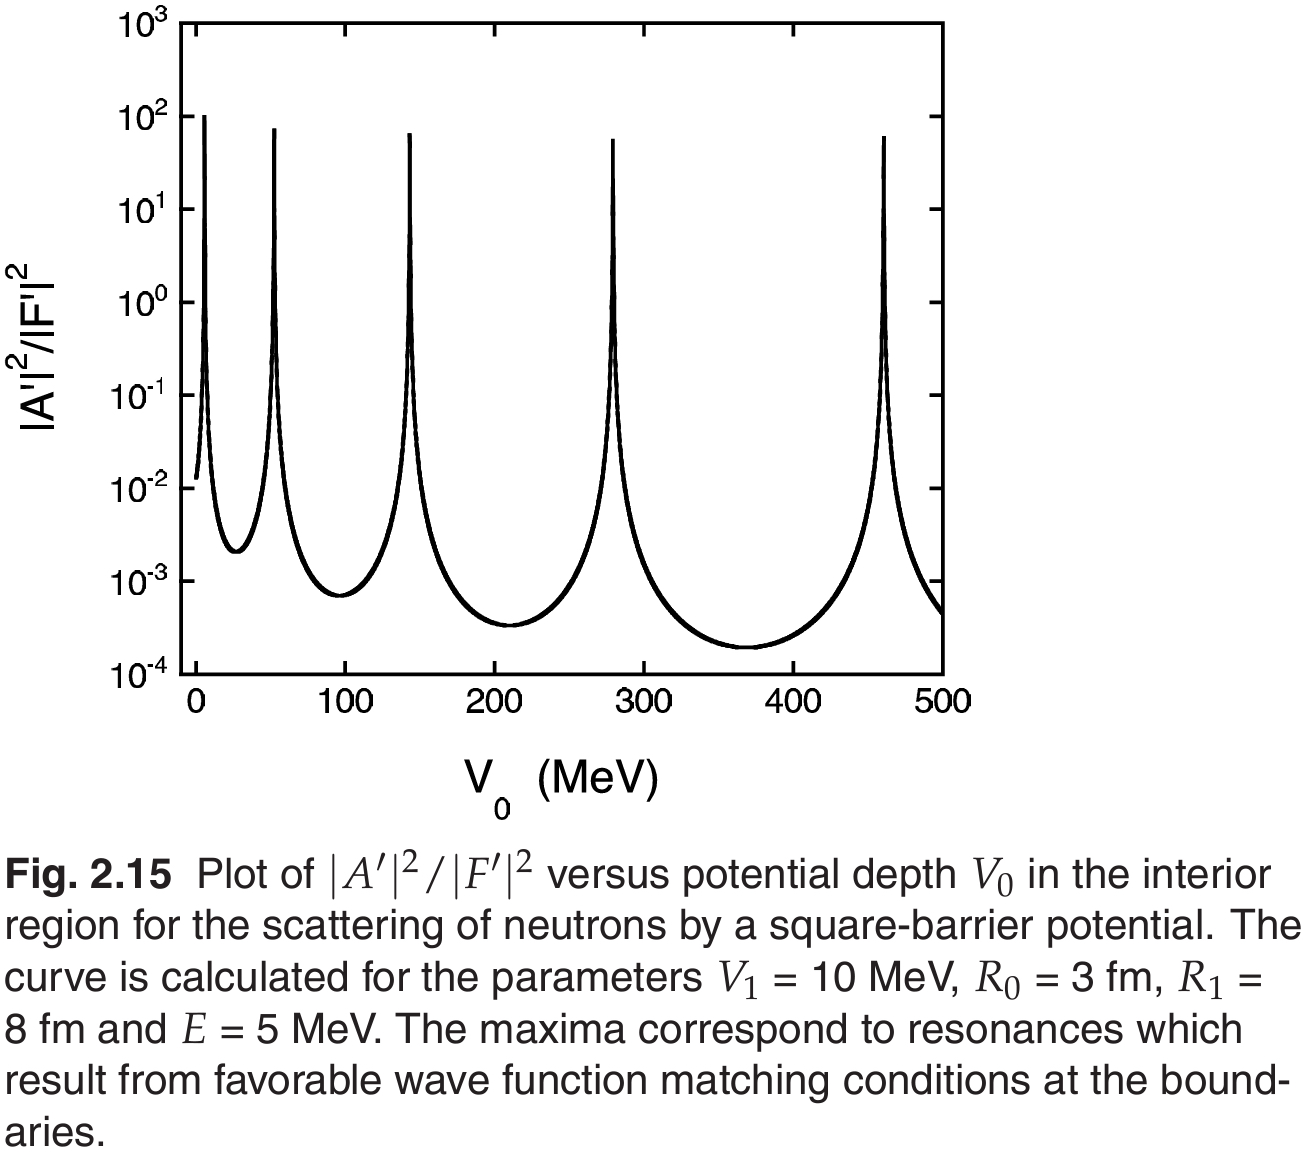
\includegraphics[trim={0.0cm 0cm 0.0cm 0},clip, keepaspectratio,width=0.9\textwidth]{A2_F2-barrier}\label{fig:A2_F2-barrier}
			\end{figure}
        \end{column}
    \end{columns}
\end{frame}

\begin{frame}{Scattering: square barrier potential transmission (1D)}
    \begin{columns}[T]
        \begin{column}{0.7\textwidth}
            \begin{align*}
                &(u_I)_{R_0}=(u_{II})_{R_0}, (\TDy{x}{u_I})_{R_0}=(\TDy{x}{u_{II}})_{R_0}\\
                &(u_{II})_{R_1}=(u_{III})_{R_1}, (\TDy{x}{u_{II}})_{R_1}=(\TDy{x}{u_{III}})_{R_1}\\
                &A\alpha\exp{iKR_0}+B\alpha^*\exp{-iKR_0}=\exp{-\kappa(R_1-R_0)}(F\beta\exp{ikR_1}+G\beta^*\exp{-ikR_1})\\
                &A\alpha^*\exp{iKR_0}+B\alpha\exp{-iKR_0}=\exp{\kappa(R_1-R_0)}(F\beta^*\exp{ikR_1}+G\beta\exp{-ikR_1})\\
                &\alpha=1+i \frac{K}{\kappa}, \beta=1+i\frac{k}{\kappa}, \Delta=R_1-R_0\\
                &B[\alpha^*\beta^*\exp{\kappa\Delta}-\alpha\beta\exp{-\kappa\Delta}]=G[(\beta^*)^2-\beta^2]\exp{-i(kR_1-KR_0)}=-2i \frac{k}{\kappa}G\exp{-i(kR_1-KR_0)}\\
                &T=\frac{K|B|^2}{k|G|^2}=\frac{4Kk/\kappa^2}{|\alpha^*\beta^*\exp{\kappa\Delta}-\alpha\beta\exp{-\kappa\Delta}|^2}\\
                &=\frac{Kk}{(k+K)^2+(\kappa^2+K^2+k^2+K^2k^2/\kappa^2)\sinh^2{\kappa\Delta}}\\
                &\frac{1}{T}=\frac{1}{\sqrt{E(E+V_0)}}[(2E+V_0+2 \sqrt{E(E+V_0)})+\\
                &+(E+V_0+V_1+\frac{E(E+V_0)}{V_1-E})\sinh^2{(\sqrt{\frac{2m}{\hbar^2}(V_1-E)}\Delta)}]\\
                &\kappa\Delta=\frac{\sqrt{2m(V_1-E)}}{\hbar}(R_1-R_0)\gg1\tag{low bombarding E/Thick barrier}\\
                &|\alpha^*\beta^*\exp{\kappa\Delta}-\alpha\beta\exp{-\kappa\Delta}|^2\approx|\alpha^*\beta^*\exp{\kappa\Delta}|^2\Rightarrow T\approx4 \frac{\sqrt{E(E+V_0)}(V_1-E)}{V_1(V_0+V_1)}\exp{-2\kappa(R_1-R_0)}\\
                &T\approx\exp{-\frac{2}{\hbar}\sqrt{2m(V_1-E)}(R_1-R_0)}\tag{Strict: neutral, $l=0$ scatt.}
            \end{align*}
        \end{column}
        \begin{column}{0.25\textwidth}
            \begin{figure}[!ht]
                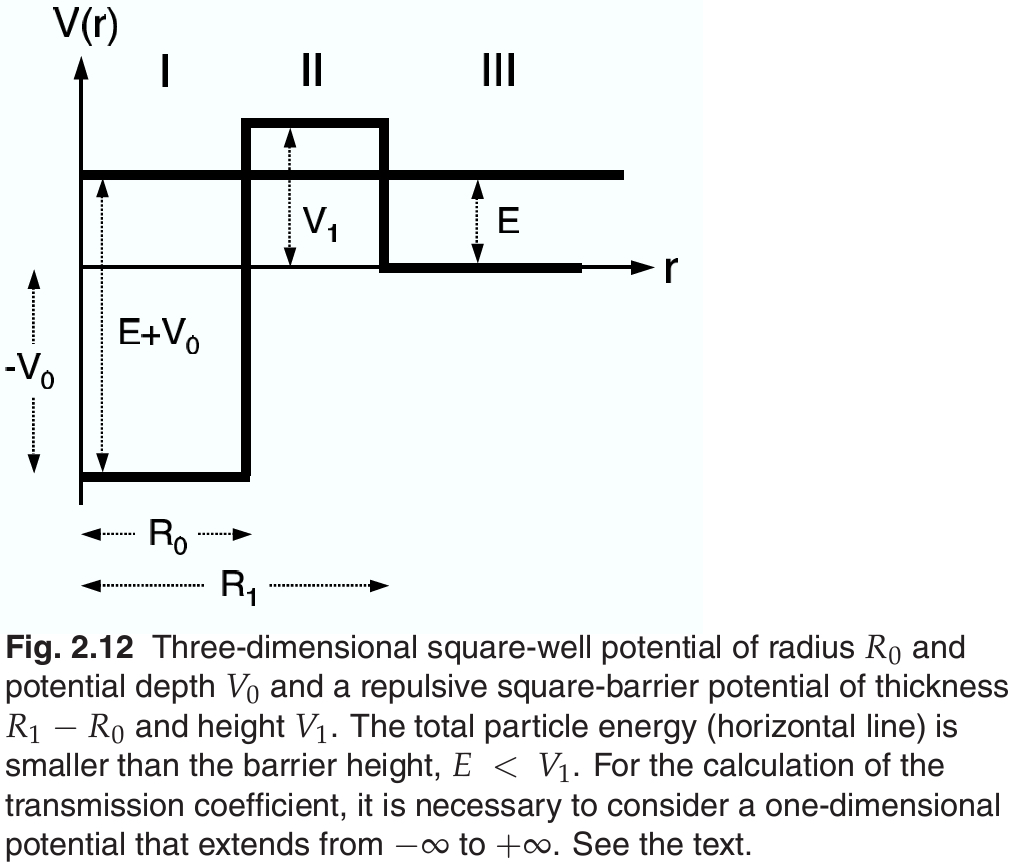
\includegraphics[trim={0.0cm 0cm 0.0cm 0},clip, keepaspectratio,width=0.8\textwidth]{nuclear-square-barrier}\label{fig:nuclear-square-barrier}
                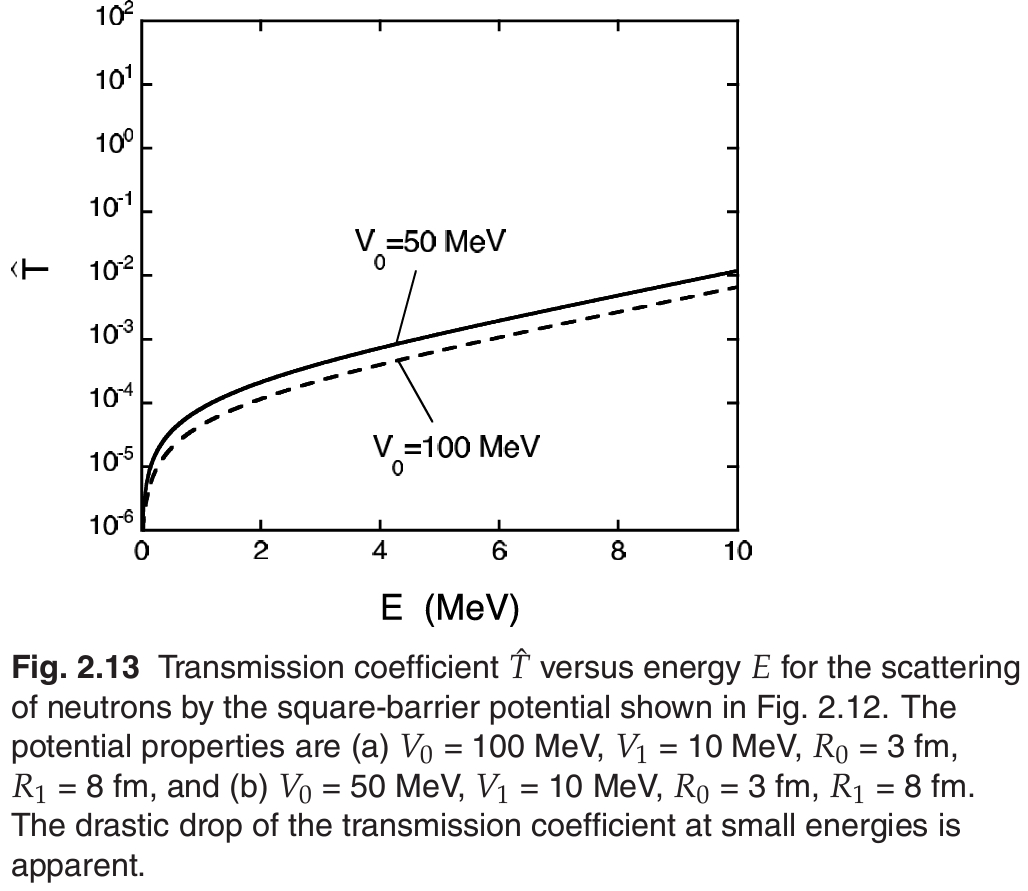
\includegraphics[trim={0.0cm 0cm 0.0cm 0},clip, keepaspectratio,width=0.8\textwidth]{transcoeff-squarebarrier}\label{fig:transcoeff-squarebarrier}
			\end{figure}
            1D radial wave-function:
            \begin{align*}
                &u_I=A\exp{iKx}+B\exp{-iKx}\\
                &u_{II}=C\exp{-\kappa x}+D\exp{\kappa x}\\
                &u_{III}=F\exp{ikx}+G\exp{-ikx}\\
                &T=\frac{j_{trans}}{j_{inc}}=\frac{K|B|^2}{k|G|^2}\\
                &A=0\tag{no wave from left}\\
                &F=0
            \end{align*}
        \end{column}
    \end{columns}
    
\end{frame}

\subsection{Opacity}

\subsection{Stellar model}

\begin{frame}{Homologous Stars: h. mass shell, $\frac{m}{M}=\frac{m'}{M'}$, are at h. points, $\frac{r}{R}=\frac{r'}{R'}$}
    \begin{columns}[T]
        \begin{column}{0.50\textwidth}
            \begin{align*}
            &\xi=\frac{m}{M}=\frac{m'}{M'}: \frac{r(\xi)}{r'({\xi})}=\frac{R}{R'}\\
                &\begin{array}{l}
                \frac{r}{r'}=z=\frac{R}{R'},\frac{P}{P'}=p=\frac{P_c}{P_c'}\\
                \frac{T}{T'}=t=\frac{T_c}{T_c'},\frac{l}{l'}=s=\frac{L}{L'}
            \end{array}\tag{Ansaz}\\
            &\begin{array}{l}
                \TDy{\xi}{r}=c_1 \frac{M}{r^2\rho},c_1=\frac{1}{4\pi}\\
                \TDy{\xi}{P}=c_2 \frac{\xi M^2}{r^4},c_2=-\frac{G}{4\pi}\\
                \TDy{\xi}{l}=\epsilon M,\TDy{\xi}{T}=c_4 \frac{\kappa lM}{r^4T^3},c_4=-\frac{3}{64\pi^2ac}
            \end{array}\\
            &\begin{array}{l}
                \TDy{\xi}{r'}=c_1 \frac{M'}{r'^2\rho'}[\frac{x}{z^3d}],\TDy{\xi}{P'}=c_2 \frac{\xi M'^2}{r'^4}[\frac{x^2}{z^4p}]\\
                \TDy{\xi}{l'}=\epsilon'M'[\frac{ex}{s}],\TDy{\xi}{T'}=c_4 \frac{\kappa'l'M'}{r'^4T'^3}[\frac{ksx}{z^4t^4}]
            \end{array}\\
            &\frac{x}{z^3d}=1, \frac{x^2}{z^4p}=1, \frac{ex}{s}=1, \frac{ksx}{z^4t^4}=1\\
            &\begin{psmallmatrix}
                -3&-\alpha&\delta&0\\
                -4&-1&0&0\\
                0&\lambda\alpha&(\nu-\lambda\delta)&-1\\
                -4&a&(b-4)&1\\
            \end{psmallmatrix}
            \begin{psmallmatrix}
                z_1\\p_1\\t_1\\s_1\\
            \end{psmallmatrix}=\begin{psmallmatrix}
                -1\\-2\\-1\\-1\\
            \end{psmallmatrix}\tag{x}\\
            &\begin{psmallmatrix}\setlength\arraycolsep{-10pt}
                -3&-\alpha&\delta&0\\
                -4&-1&0&0\\
                0&\lambda\alpha&(\nu-\lambda\delta)&-1\\
                -4&a&(b-4)&1\\
            \end{psmallmatrix}
            \begin{psmallmatrix}
                z_2\\p_2\\t_2\\s_2\\
            \end{psmallmatrix}=\begin{psmallmatrix}
               \phi\\0\\-\lambda\phi\\0\\
            \end{psmallmatrix}\tag{y}
             \end{align*}
        \end{column}
        \begin{column}{0.50\textwidth}
            \begin{itemize}
                \item exponents solutions:
    \begin{align*}
            &z_1=\frac{1}{2}(1+A),p_1=-2A,t_1=\frac{1}{2\delta}[1+(3-4\alpha)A],\\
            &s_1=1+\frac{4-b}{2\delta}+[2+2a+\frac{3-4\alpha}{2\delta}(4-b)]A\\
            &z_2=\phi B,p_2=-4\phi B,t_2=\frac{\phi}{\delta}[1+(3-4\alpha)B],\\
            &s_2=\frac{\phi}{\delta}(4-b)+\phi[4+4a+\frac{3-4\alpha}{\delta}(4-b)]B\\
            &A=\invers{[\frac{4\delta(1+a+\lambda a)}{\nu+b-4-\lambda\delta}+4\alpha-3]},\\
            &B=A\invers{(1-\frac{\lambda\delta}{\nu+b-4})}\\
            &\frac{x}{z^3d}=1\Rightarrow \frac{\rho}{\rho'}=\frac{M/M'}{(R/R')^3},\frac{x^2}{z^4p}=1\\
            &\Rightarrow \frac{P}{P'}=\frac{(M/M')^2}{(R/R')^4}
    \end{align*}
    
\end{itemize}    
        \end{column}
    \end{columns}
    \begin{itemize}
    \item $\delta=0$ polytropic: $n=\frac{\alpha}{1-\alpha}$, $A=\invers{(4\alpha-1)}$, $z_1=\frac{2\alpha-1}{4\alpha-3}$, $R\propto M^{z_1} (MR-rel, $y=1$, $\alpha=\frac{3}{5}$ (NR \Pelectron gas): $z_1=-\frac{1}{3}$
    \item Ideal gas, const $\kappa$ - $\alpha=\delta=\phi=1$, $a=b=0$ - $ML$, $L\mu$ rel: $\frac{L}{L'}=(\frac{M}{M'})^3(\frac{\mu}{\mu'})^4$: $z_1=\frac{\nu+\lambda-2}{\nu+3\lambda}$, $z_2=\frac{\nu-4}{\nu+3\lambda}$, $p_1=2-4z_1$, $p_2=-4z_2$, $t_1=1-z_1$, $t_2=1-z_2$, $s_1=3$, $s_2=4$; $\frac{R}{R'}=(\frac{M}{M'})^{z_1}$ ($\frac{\mu}{\mu'})^{z_2}$ ($z_1\in\numrange{0.4}{0.8}$).
    \end{itemize}
\end{frame}

\begin{frame}{Solution for exponents of x,y and applications to simple material functions}
    \begin{align*}
            &z_1=\frac{1}{2}(1+A),p_1=-2A,t_1=\frac{1}{2\delta}[1+(3-4\alpha)A],s_1=1+\frac{4-b}{2\delta}+[2+2a+\frac{3-4\alpha}{2\delta}(4-b)]A\\
            &z_2=\phi B,p_2=-4\phi B,t_2=\frac{\phi}{\delta}[1+(3-4\alpha)B],s_2=\frac{\phi}{\delta}(4-b)+\phi[4+4a+\frac{3-4\alpha}{\delta}(4-b)]B\\
            &A=\invers{[\frac{4\delta(1+a+\lambda a)}{\nu+b-4-\lambda\delta}+4\alpha-3]},B=A\invers{(1-\frac{\lambda\delta}{\nu+b-4})}\\
            &\frac{x}{z^3d}=1\Rightarrow \frac{\rho}{\rho'}=\frac{M/M'}{(R/R')^3},\frac{x^2}{z^4p}=1\Rightarrow \frac{P}{P'}=\frac{(M/M')^2}{(R/R')^4}\tag{H. points: $\frac{r}{r'}=z$, $\xi=\frac{m}{M}=\frac{m'}{M'}$, $\frac{r(\xi)}{r'(\xi)}=\frac{R}{R'}$}
    \end{align*}
For all h. points density changes as mean density while $P\propto M^2R^{-4}$.
\begin{columns}[T]
    \begin{column}{0.3\textwidth}
        \begin{block}{$\delta=0$: polytropic}
            \begin{align*}
                &n=\frac{\alpha}{1-\alpha}\\
                &A=\invers{(4\alpha-1)}\\
                &z_1=\frac{2\alpha-1}{4\alpha-3}\\
                &R\propto M^{z_1}\tag{MR-rel, $y=1$}\\
                &\alpha=\frac{3}{5}:\tag{NR \Pelectron gas}\\
                &z_1=-\frac{1}{3}
            \end{align*}
        \end{block}
    \end{column}
    \begin{column}{0.38\textwidth}
        \begin{block}{Ideal gas, const $\kappa$: $\alpha=\delta=\phi=1$, $a=b=0$}
            \begin{align*}
                &z_1=\frac{\nu+\lambda-2}{\nu+3\lambda},z_2=\frac{\nu-4}{\nu+3\lambda}\\
                &p_1=2-4z_1,p_2=-4z_2\\
                &t_1=1-z_1,t_2=1-z_2\\
                &s_1=3,s_2=4\\
                &\Rightarrow \frac{L}{L'}=(\frac{M}{M'})^3(\frac{\mu}{\mu'})^4\tag{$ML$,$L\mu$ rel}\\
                &\frac{R}{R'}=(\frac{M}{M'})^{z_1}(\frac{\mu}{\mu'})^{z_2}\tag{$z_1\in\numrange{0.4}{0.8}$}
            \end{align*}

        \end{block}
    \end{column}
    \begin{column}{0.32\textwidth}
        \begin{block}{Approx constant $P_{rad}$}
                If material functions don't contain only product: 
            \begin{align*}
                &\rho=(\mu\beta)\frac{P}{T},\beta=\frac{P_g}{P}=1-\frac{P_r}{P}\\
                &R\propto\beta^{z_2},P\propto\beta^{p_2}\\
                &T\propto\beta^{t_2},L\propto\beta^{s_2}\tag{$\beta$ det. by $P,T$}\\
                &1-\beta=\frac{P_r}{P}\propto \frac{T^4}{P}\propto\frac{M^{4t_1}}{M^{p_1}}\frac{\beta^{4t_2}}{\beta^{p_2}}\\
                &\frac{1-\beta}{\beta^4}\propto M^2\tag{replacing expression for exponent}
            \end{align*}
        \end{block}
    \end{column}
\end{columns}
\end{frame}

\begin{frame}{Homologous contraction (poly index n)}
    Consecutive models are h. to each others, ie contraction of polytrope that doesn't change polytropic index; $z\propto\frac{r}{R}$ dim-less radius var: LE eqs gives $m(z)$ so mass elements at homologous points, mass elements ($\xi=\frac{m}{M}=\const{}$) remains at h. points, since their value of z do not change in time.
\begin{align*}
&r'=r+\dot{r}\Delta t\Rightarrow\frac{r}{r'}=1+\frac{\dot{r}}{r}\Delta t\\
&\frac{r'}{r}=\frac{R'}{R}=\const{}\Rightarrow\frac{\dot{r}}{r}=\frac{\dot{R}}{R}=\const{}\ (\PDof{m}\PDy{t}{\ln{r}})=0\\
&\PDof{t}(\frac{1}{r}\PDy{m}{r})=0=\PDof{t}(\frac{1}{4\pi r^3\rho})\Rightarrow\frac{\dot{\rho}}{\rho}=-3\frac{\dot{r}}{r}\\
&P=\int_m^M\frac{Gm}{4\pi r^4}\,dm:\ \dot{P}=\int_m^M\PDof{t}(\frac{1}{r^4})\frac{Gm}{4\pi}\tag{HE}\\
&\rho\propto P^{\alpha}T^{-\delta}\Rightarrow\frac{\dot{\rho}}{\rho}=\alpha\frac{\dot{P}}{P}-\delta\frac{\dot{T}}{T}\tag{EOS}\\
&\frac{\dot{T}}{T}=-\frac{4\alpha-3}{\delta}\frac{\dot{r}}{r}\\
&\epsilon_g=c_PT(\nad\frac{\dot{P}}{P}-\frac{\dot{T}}{T})=c_PT[-4\nad+\frac{4\alpha-3}{\delta}]\frac{\dot{R}}{R}\\
&\to-\frac{3}{5}c_PT\frac{\dot{R}}{R}\tag{ideal mono $\nad=\frac{2}{5}$, $\alpha=\delta=1$}\\
\end{align*}
\end{frame}

\subsection{Fato Finale}

\begin{frame}{Post AGB}
    \begin{itemize}
        \item $M_*>\numrange{8}{10}\msun{}$: core He-burning produces compact CO core - Limit $M_{up}$ is largest mass where electron degeneracy of CO core prevent C-burning; $M>M_{up}$ massive stars, stars igniting He-burning in non-deg core but developing deg CO core are int-mass star.
        \item $M<_{up}$: thermally pulsating AGB. TPAGB terminated when CO mass exceds limit $M_{ch}\approx1.4\msun{}$ and Carbon ignites, or mass H-rich envelope is exhausted. Due to mass loss is not expected CO core reaches Ch. limit in TPAGB phase.
        \item AGB mass loss obs: \numrange{e-8}{e-4}$\msun{}\si{\per\year}$. Mira variables-radiation driven wind;
            \begin{columns}[T]
                \begin{column}{0.5\textwidth}
                    \begin{align*}
                        &\log{(\TDy{t}{M})}=-11.4+0.0123\log{P}\tag{$P<\SI{500}{\day}$}\\
                        &\TDy{t}{M}=\num{6.07023e-3}\frac{L}{cv_e}\tag{$P>\SI{500}{\day}$}
                    \end{align*}
                \end{column}
                \begin{column}{0.5\textwidth}
                    \begin{align*}
                        &v_e=-13.5+0.056P\tag{term.vel.stellar wind \si{\kilo\meter\per\second}}\\
                        &\log{P}=-2.07+1.94\log{R}-0.9\log{M}\tag{\si{\day}}
                    \end{align*}
                \end{column}
            \end{columns}
            
        \item Evolution of low mass stars after TPAGB/formation of Planetary Nebula (when $T_e\approx \SI{30000}{\kelvin}$ ejected materials is ionized): once mass H-rich envelope below critical value star evolve rapidly toward hotter $T_e$: burn H until bluest point in thin shell at almost const L, then H-burning switch off and both H-,He-rich envelopes contract rapidly. Dep on thermal condition of envelope: nuclear burning dies and remnant cools as WD; Heating of He-rich layers leads to He-runaway-burning bringing back to AGB (born-again AGB: FG sagittae) and moving to blu side until WD; heatin of H-rich envelope induce H-burning in runaway manner (selfinduced nova), violent explosion of H-rich envelope (DB WD), if only part of H-rich envelope is lost we may have more H-flashes ending again with non-DA WD.
    \end{itemize}
\end{frame}

\begin{frame}{WD cooling}
    
\end{frame}

\begin{frame}{Massive stars: $M>M_{up}$ - neutrino mediated KH contraction of CO core}
    \begin{itemize}
        \item Similar evolution but sensitivity of location on HDR to mass-loss and convection (Sch vs Ledoux: affects ratio between time spent on blu/red side of HDR).
        \item Mass of He core is fixed by mass-size of convective core during central H-burning and amount of hydrogen processed in H-burning shell during central He-burning stage: mass of CO core quite fixed size of convective core during central He-burning phase (H-burning phase is fast, chem profile of C/O are flat in core as result of efficient mixing in He-burning phase).
        \item C abundance in core affects successive phase: sensitive to cross section of $^{12}C(\alpha,\gamma)^{16}O$
        \item At central He exhaustion CO begins contract; $T_c\geq\SI{5e8}{\kelvin}$ entering region of $\rho_c-T_c$ plane where neutrino losses from pair annihilation dominates stellar energy budget - radiative/convective energy transport are still important for stellar structure but is neutrino luminosity that balance energy by contraction and nuclear burning.
        \item For $M=\numrange{15}{30}\msun{}$ C-burning ignites when $T_c=\SIrange{0.3e9}{1.2e9}{\kelvin}$ via $^{12}C+^{12}C\to^{24}Mg$ highly excited, decaying as $^{24}Mg\to^{23}Mg+n$ or $\to^{20}Ne+\alpha$ or $^{23}Na+p$. Abundance of C determine whether convective core is formed: nuclear rate minus neutrino luminosity must be positive ($\PDy{m}{l}=\epsilon_n+\epsilon_g-\epsilon_{\nu}$). Decrease of CC-mass with increasing stellar mass: \xaumenta{M}, \xaumenta{T_c}, \xaumenta{\epsilon_{\nu}}, so for large stellar mass CC disappears (could break corr. between CC-mass and central $X_C$). Once C is exhausted C-burning shift quitely in shell (we have one or more convective episode in C burning regions??); during C-burning (part. in shell) sign. fractioin of s-el are produced(most eff. neutron source in this phase is $^{22}Ne(\alpha,n)^{25}Mg$).
    \end{itemize}
\end{frame}

\begin{frame}{Massive stars: $M>M_{up}$ - Ne,O,Si-burning}
    \begin{itemize}
        \item Ne-Burning: after C-burning composition is $X_{^{16}O}\approx0.7$, $X_{^{20}Ne}\approx\numrange{0.2}{0.3}$, $^{24}Mg$; oxygen has lowest Coulomb barrier but before endpothermic reaction $^{20}Ne(\gamma,\alpha)^{16}O$ is allowed as high energy photons; whole set exothermic reactions during this phase make Ne-burning via $^{20}Ne(\gamma,\alpha)^{16}O$ exothermic for $T_c\approx\SIrange{1.2}{1.9}{\giga\kelvin}$.
            CC is always formed but exists for short time during which nuclear rate exeeds neutrino loss, when central Ne is exhausted Ne-burning shift in shell.
        \item O-Burning: At end of Ne-burning composition is $^{16}O$, $^{24}Mg$, $^{28}Si$. For $M\approx\num{15}{30}\msun$ O-burning at $T_c\approx\SIrange{1.5}{2.6}{\giga\kelvin}$. $^{16}O+^{16}O\to^{32}S$, $^{32}S\to^{31}S+n$, $^{32}S\to^{31}P+p$, $^{32}S\to^{30}P+^2D$ inhibited at low T while at high T D is photodis, $^{32}S\to^{28}Si+\alpha$. CC of $1\msun$ regardless of total stellar mass. O-burning so short, and from now on, that star is frozen. Due to large eff. of weak interaction, $^{30}P(\APelectron,\Pnu)^{30}S$, $^{35}Cl(\Pelectron,\nu)^{35}S$, $^{37}Ar(\Pelectron,\Pnu)^{37}Cl$, pneutron rich nuclei are produced, neutronization level increases. At O exhaustion O-burning moves in shell with one or more convective episode. Near end of burning for $T_c\approx\SIrange{2.5}{2.8}{\giga\kelvin}$ exist quasi-equilibrium clusters where reactions are balanced by their inverse, ie $^{29}Si(p,\gamma)^{30}P$.
        \item Si-Burning: $T_c\approx\SI{2.3e9}{\kelvin}$. Photodisintegration chain: $^{28}Si(\gamma,\alpha)^{24}Mg(\gamma,\alpha)^{20}Ne(\gamma,\alpha)^{16}O(\gamma,\alpha)^{12}C(\gamma,2\alpha)\alpha$, strongly affected by level of neutronization. Two distinct episode: radiative and convective, during first $^{28}Si\to^{30}Si$, the lower the mass the more complete $^{28}Si$-destruction is. When nuclear generation overcomes neutrino losses (no more dominated by pair production but weak interactions, ie \Pelectron-capture on heavy elements), appears CC, approx $1\msun$ indep of stellar mass; during CC \xaumenta{X_{^{28}Si}} as convection penetrates in richer regions due to O-burning. At end of Si-burning core is made of $^{56}Fe$, $^{52}Cr$. At exhaustion of Si, burning moves in shell where we have recurrent convective episodes whose extensios set the limit between matter with high/low level of neutronization: set mass of so called iron-core - the lower the mass of iron core, the larger probability of explosion. The last reaction to achieve equilibrium is $3\alpha$ which finally occurs at rate balancing C-photo-diss.: NSE is achieved.
    \end{itemize}
\end{frame}

\begin{frame}{Core collapse SN (type II SN)}
    \begin{itemize}
        \item Stable configuration for $\gamma=\frac{c_P}{c_v}>\frac{4}{3}$ (virial T.); in core of massive stars after NSE, both photodisintegration and relativistic effects decrease $\gamma$ below $\frac{4}{3}$ and core begins collapse.
        \item At beginning collapse occurs in $\tkh{}$ due to huge \Pnu flux which carries away core binding energy.
    \item Two instabilities causes collapse acceleration: i) due to increase in density neutronization process becomes increasingly efficient: this process removes free electrons which are main pressure contributors, ii) photo-disintegration becomes more efficient producing large number of $\alpha$ particles. The binding energy of the core resulting from this new composition is lower than before, and so star can't gain enough energy from contraction: collapse accelerate.
\item Collapse last few ms deps on initial core density. When density \SI{e14}{\gram\per\cubic\cm}, NS density, material becomes incompressible and collapse in central regions stops. Core rebounds and supersonic impact with external layers produce shockwave. Prompt explosion scenario: in perfectly elastic collision: kinetic energy \SIrange{e52}{e53}{\erg} of rebounding core vs binding energy of outer envelope \SIrange{e50}{e51}{\erg} - this is impossible as energy is dissipated by photo-disintegration due to heating of material induced by shockwave (\SI{e51}{\erg} per $0.1\msun$ crossed), as emission of neutrino from behind shockwave is efficient cooling process.
\item Neutrino powered explosion: due to high density of core mean free path of neutrinos, produced by neutronization processes, becomes comp. to core radius; with increasing density neutrinos experience multiple scattering and in inner core density is so high that neutrinos diffusion velocity is smaller than collapse velocity (it's called neutrino-trapping-surface where we have equal velocity). For $M_*<25\msun{}$ can be produced a NS of mass equals to iron core.
\item Pair-instability SN: $M_*>100\msun{}$, or $M_{HeC}>40\msun{}$ (Pop.III stars). After He burning we have positron-electron pair reducing $\gamma<\frac{4}{3}$ and collapse producing prompt explosion en BH.
\item explosive burning determined by temperature(/how long) of shockwave, change isotopic ratio for O, Si, Ne, C burning; significant production of $^7Li$, $^{11}B$, $^{19}F$, $^{26}Al$ via neutrino processes. Most massive can produce r-elements. Main contributor of $\alpha$-elements: O, Ne, Mg, Si, S, Ca, Ti. 
    \end{itemize}
\end{frame}

\begin{frame}{Type Ia SN: progenitors}
    \begin{itemize}
        \item SN Ia comes from CO WD accreting mass from companion until mass is enough to trigger runaway thermonuclear reaction; type Ib,Ic SN are thought as explosive ending of massive stars that have lost whole H-rich envelope.
        \item Spectral classification. Type I: no H features (upper limit to H abundance is \SI{e-4}{\solarmass}); Ia: SiII absorption line \SI{6150}{\angstrom}, late spectra shows many Fe emission lines; Ib,Ic: no SiII absorption lines, presence/not of strong He I lines at \SI{5876}{\angstrom}.
\item SN Ia progenitors - For $M<M_{up}$ star develop degenerate CO core turning into WD and if has a companion will accretes materials and we'll have different channel as different initial mass, chemical composition and accretion rate: a) DD-scenario. Accretion of H-rich materials (also classical/symbiontic nova) within system formed by 2 int-mass star, ie Double Degenerate scenario, evolving through episode of common envelope, and a system of two CO WD finally forming object with $M>M_{Ch}$ which can't be in hydrostatic equilibrium - Lack of observed DD systems. b) Single Degenerate scenario: accretion of H-/He-rich materials at appropriate rate - i) Accretion of H-rich matter on massive WD $\approx 1\msun{}$ with as low accretion as $\TDy{t}{M}\leq \num{e-9}\msun{}\si{\per\year}$ increasing mass of WD through strong He-pulses above $M_{Ch}$ but much mass is ejected so take Hubble time to reach $M_{Ch}$ (H-burning on top of He layer is so slow that He-shell develop strong degeneracy); at larger accretion rate star can explode: peculiar explosive nucleosynthesis and large H abundance should  be observable in early spectra, which is incompatible with SN Ia observation (however it's improb. to observe WD with initial mass larger than $1.1\msun{}$: progenitors could ignite CO core-WD config.); c) Sub-Chandrasekhar scenario. Considering low-mass CO WD accreting H-rich materials $\approx\num{3e-8}\msun{}\si{\per\year}$ can deliver thermon. explosion delivering \SI{e51}{\erg}, typical of SNIa (violent He-ignition after accretion of $0.15\msun{}$, ie when a very cold accreting WD reaches \SIrange{0.65}{0.8}{\solarmass}: if WD initially massive enough  He-burning could result in detonation and inward moving compression wave could lead to detonation of carbon in core); d) for H-accretion rate near Eddington limit accreted materials achieve expanded configuration typic. of RGB stars (Eddington Luminosity: max surface luminosity of star with outer layers in rad-equil: $L_{Edd}\propto \frac{M}{\kappa}$).
    \end{itemize}
\end{frame}

\begin{frame}{SN type I: spectral features}
    \begin{itemize}
\item SN type Ia have same spectrum and light curve; big distance standard candle.
        \item SN Ia comes from CO WD accreting mass from companion until mass is enough to trigger runaway thermonuclear reaction; type Ib,Ic SN are thought as explosive ending of massive stars that have lost whole H-rich envelope.
        \item Spectral classification. Type I: no H features (upper limit to H abundance is \SI{e-4}{\solarmass}); Ia: SiII absorption line \SI{6150}{\angstrom}, late spectra shows many Fe emission lines; Ib,Ic: no SiII absorption lines, presence/not of strong He I lines at \SI{5876}{\angstrom}.
        \item Comm. used feature of type Ia SN light curves is max brightness in optical B band - steep rise approx \SI{0.5}{\mag\per\day} in about \SIrange{10}{18}{\day}; then becomes slowly in near-UV and optical B-band, at longer wavelength is different: in V band fading slows down after \SI{20}{\day}, in R-band plateau, in IJHK-bands a secondary maximum occurs, after \SI{50}{\day} SN fades away monot. in all bands.
        \item Significative deps. of light curves characteristic on p-band is evidence of interaction between ejecta and radiative flux.
        \item SN Ia as distance indicators - Constance of max B magnitude (almost: scatter \SIrange{0.2}{0.4}{\mag}). Invariance: a) linear corr. between abs. mag at max and decline rate $\Delta m_{15}$, magnitude diff max-max+15d: $M_B=-21.726+2.698\Delta m_{15}(B)$, $\cdots$. Above and similar allowed usage of SN Ia as distance indicator.
    \item Light curves of SN Ia are powered by decay of $^56Ni$ and its daughter $^{56}Co$, $^{56}Ni$ is during explosive burning and decay with $t_{\frac{1}{2}}$=\SI{6.1}{\day} to $^{56}Co$, $^{56}Co\to ^{56}Fe$ via electron-capture/$\beta^+$-decay with $t_{\frac{1}{2}}=\SI{77}{\day}$, during late phase light curve deps also on \APelectron (from minor channel of $^{56}Co$) annihilated in ejecta after losing their kin. ener.
    \end{itemize}
\end{frame}

\begin{frame}{Explosion Models}
    \begin{itemize}
        \item Properties of explosion depend on how shockwave propagates inside WD: different between Chandra vs sub-Chandra progenitor.
        \item Energy delivery: \SI{e51}{\erg}
        \item Nucleasynthesis of \SIrange{0.4}{1.0}{\solarmass} of $^{56}Ni$ to power lightcurve.
        \item Production of significant amount of intermediate-mass elements expanding at \SI{10000}{\kilo\meter\per\second}
\item Chandra progenitor - C ignited in central regions for $\rho\approx\SI{e9}{\gram\per\cubic\cm}$: due to high degeneration is explosive and incinerate Fe-peak elements; explosive burning flames propagate outward - subsonic: deflagration - properties of propagation are influenced by instabilities, behind flame front Si, O, Ne, C burn explosiv.: composition of processed materials deps on T and $\rho$ of burning front - for $\rho\approx\SIrange{e10}{e6}{\gram\per\cubic\cm}$ burnt materials ranges from Fe-peak elements (mainly $^{56}Ni$) to interm.-mass elements such S, Si, and in more external layers, C,O. The flame encounters regions whose density could be lowered by WD expansion: resulting explosive nuclesynthesis depend on flame's velocity: i) deflagration to detonation (supersonic) due to compression shock crossing low-density outer layers - explaining extremely bright SN (SN1991T) as they for larger amount of $^{56}Ni$. ii) delayed detonation: flame speed is so low that little amount of $^{56}Ni$ (\SI{0.1}{\solarmass}), def-det transition occurs at densities \SI{e7}{\gram\per\cubic\cm} when star has expanded sign. (better fit to observed velocities of int-mass elements). iii) Pulsating-delayed-detonation: if speed of initial flame is low burning is quenched by expansion of outer layer before binding energy of structure becomes positive: WD remains bound and experiences strong pulsations - at max compression burning can re-ignite siupersonic. becoming a detonation. Better reproduct. of velocities of int-mass elements.
\item Sub-Chandra progenitor - Central explosive C burning (detonation) induced by shockwave generated by He-detonation on top of CO-core.
    \end{itemize}
\end{frame}

\subsection{Stars Formation}

\begin{frame}{Isothermal cloud structure}
    \begin{align*}
        &-\frac{1}{\rho}\nabla P-\nabla\phi_g=0, P=\rho a_T^2\Rightarrow \ln{\rho}+\frac{\phi_g}{a_T^2}=\const{}:\rho=\rho_c\exp{-\frac{\phi_g}{a_T^2}}\\
        &\xi=\sqrt{\frac{4\pi G\rho_c}{a_T^2}}r, \psi=\frac{\phi_g}{a_T^2}\Rightarrow \frac{1}{\xi^2}\TDof{\xi}(\xi^2\TDy{\xi}{\psi})=\exp{-\psi}\\
        &\xi\gg1: \frac{\rho}{\rho_c}\to \frac{2}{\xi}\Rightarrow \psi=\ln{\frac{\xi^2}{2}}, \rho(r)=\frac{a_T^2}{2\pi Gr^2},\rho_0=\frac{P_0}{a_T^2}, r_0=\frac{\xi_0}{\sqrt{\frac{4\pi G\rho_c}{a_T^2}}}\tag{SIS: large distance}\\
        &M=4\pi\int_0^{r_0}\rho r^2\,dr= 4\pi\rho_c(\frac{a_T^2}{4\pi G\rho_c})^{\frac{3}{2}}\int_0^{\xi_0}\exp{-\psi}\xi^2\,d\xi\\
        &\omega^2=k^2a_T^2-4\pi G\rho_0\Rightarrow \lambda_J=\sqrt{\frac{\pi a_T^2}{G\rho_0}}=\SI{0.19}{\parsec}\sqrt{\frac{T}{\SI{10}{\kelvin}}}(\frac{n_{H_2}}{\SI{e4}{\per\cubic\cm}})^{-\frac{1}{2}}: M_J=M_{BE}=\frac{\overbrace{m_1}^{1.18} a_T^4}{P_0^{\frac{1}{2}}G^{\frac{3}{2}}}\tag{G. stability}
    \end{align*}
\end{frame}

\begin{frame}{Protostars: structure}
    
\end{frame}

\begin{frame}{Protostars: deuterium thermostat}
    
\end{frame}

\subsection{Model computation}

 \subsection{Sun model and helioseism}

\subsection{Composition: initial params and evolution}

\begin{frame}{programma per questa sezione}
    \begin{itemize}
        \item Def Z etc composizione solare, BBN: 210216
        \item Structural deps on composition: 20210315
        \item Composizione e opacit\'a/T: 20210326, 20210329, 20210330, 20210426
        \item CNO burning
        \item processi s
        \item produzione elementi pesanti:20210420
        \item Zams: variazione con comp: 20210503
        \item Helium to metal enrichment $\frac{\Delta Y}{\Delta Z}$, broadening observed MS
        \item Dredge-up: 20210507
        \item diffusione: 20210507
        \item Deps tip rgb on comp: 20210512
        \item Deps on chem of vertical/horizontal method: 20210517
        \item R param deps on Y: 20210521
        \item DredgeUpII: 20210521
        \item DredgeUpIII: 20210524
    \end{itemize}
\end{frame}

\subsection{Polytropic}

\subsection{Homologous stars}

\begin{frame}{H.models}
\begin{itemize}
    \item  Homologus star:they have the same $\frac{T}{T_c}$, $\frac{P}{P_c}$, $\frac{\rho}{\rho_c}$ when expressed in terms of $\frac{r}{R}$.
\end{itemize}
    
\end{frame}

\subsection{Grandezze Fondamentali}\linkdest{succo}

\begin{frame}{Stime Euristiche: Tempo scala, Pressione e Temperatura centrali}
    \begin{columns}[T]
        \begin{column}{0.5\textwidth}
            \begin{align*}
                &\PDy{m}{P}=-\frac{Gm}{4\pi r^4}\Rightarrow \frac{P_0-P_c}{M}\approx \frac{2G(M/2)^2}{4\pi(R/2)^4}\\
                &\Rightarrow P_c\approx \frac{2GM^2}{\pi R^4}\\
                &\rho\xrightarrow{\text{ideal g.}}\frac{\mu}{R}\frac{P}{T}\Rightarrow T_c\approx \frac{P_c}{\rho_c}\frac{\mu}{R}\\
                &=P_c\frac{\mu}{R}\underbrace{\frac{\bar{\rho}}{\rho_c}}_{\approx0.01-0.03}\Rightarrow T_c<\frac{8}{3}\frac{G\mu}{R}\frac{M}{R}
            \end{align*}
        \end{column}
        \begin{column}{0.5\textwidth}
            \begin{align*}
                &f_P=-\PDy{m}{P}\,dm\\
                &f_g=-\frac{g\,dm}{4\pi r^2}=-\frac{Gm}{r^2}\frac{dm}{4\pi r^2}\\
                &\frac{dm}{4\pi r^2}\PtwoDy{t}{r}=f_P+f_g\Rightarrow \frac{1}{4\pi r^2}\PtwoDy{t}{r}=-\PDy{m}{P}-\frac{Gm}{4\pi r^4}\\
                &|\PtwoDy{t}{r}|\to \frac{R}{\tau_{ff}}\Rightarrow \frac{R}{\tau_{ff}}\approx g\Rightarrow\tau_{ff}\approx\sqrt{\frac{R}{g}}\\
                &\to \frac{R}{\tau_{expl}^2}\Rightarrow \frac{R}{\tau_{expl}^2}=\frac{P}{\rho R}=4\pi r^2\PDy{m}{P}=\PDy{m}{P}/\rho\\
                &\Rightarrow\tau_{expl}\approx R\sqrt{\frac{\rho}{P}}
            \end{align*}
        \end{column}
    \end{columns}
R\end{frame}

\begin{frame}{Masse limite}
    \begin{itemize}
        \item $M_{up}$: Highest *-mass at which \Pelectron-degeneracy prevent C-ignition in CO core. Depends strongly on chem. composition - $M_{up}\approx8\msun{}$ at solar metallicity.
    \end{itemize}
\end{frame}

\subsection{Equazioni struttura: Energy transport}

\begin{frame}{Radiative transport}
    \begin{columns}[T]
        \begin{column}{0.5\textwidth}
            \begin{align*}
                &I(\theta)\,d\Omega=cu(\theta)\,d\Omega\\
                &u=\int^{4\pi}u(\theta)\,d\Omega=\frac{1}{c}\int I(\theta)\,d\Omega\tag{Energy density}\\
                &J(\vec{r},\nu,t)=\invers{(4\pi)}\int I(\vec{r},\hat{n},\nu,t)\,d\Omega\tag{Mean Intensity}\\
                &P_r=\frac{1}{3}\int_0^{\infty}\frac{h\nu}{c}cn(\nu)\,d\nu=\frac{1}{3}u\tag{rad Press}\\
                &P_r=\frac{1}{c}\int I(\theta)\cos^2{\theta}\,d\Omega\tag{Rad Press}\\
                &=\int^{4\pi}\frac{I(\theta)\cos{\theta}}{c}\cos{\theta}\,d\Omega\\
                &=\frac{2\pi}{c}\int_0^{2\pi}I(\theta)\cos{\theta}\sin{\theta}\,d\theta\\
                &H=\int I(\theta)\cos{\theta}\,d\Omega\\
                &=2\pi\int_0^{\pi}I(\theta)\cos{\theta}\sin{\theta}\,d\theta\tag{Net En. Flux polar dir}
            \end{align*}
        \end{column}
        \begin{column}{0.4\textwidth}
            Pressione di radiazione: radiazione contenuta in parallelepipedo di superficie unitaria lunghezza c in direzione $\theta$ (l'asse polare forma con la radiazione un angolo $\theta$) quindi la sezione d'urto geometrica in direzione polare contiene fattore $\cos{\theta}$, la proiezione del momento rispetto alla direzione polare ha un altro $\cos{\theta}$.
        \end{column}
    \end{columns}
\end{frame}

\begin{frame}{Flusso di energia proporzionale al gradiente termico}
\begin{block}{Diffusion Approx: Stellar Interior Near TE}
    \begin{columns}[T]
        \begin{column}{0.5\textwidth}
    \begin{align*}
                &U=aT^4\\
                &''\vec{j}=-D\nabla n''\tag{diffusion}\\
                &D=\frac{1}{3}vl_p\\
                &\vec{F}_{\nu}=-D_{\nu}\nabla U_{\nu}\\
                &D_{\nu}=\frac{1}{3}cl_{\nu}=\frac{c}{3\kappa_{\nu}}\rho
            \end{align*}
        \end{column}
        \begin{column}{0.5\textwidth}
            \begin{align*}
                &I(\theta)=I_0+I_1\cos{\theta}+\ldots\\
                &u=\frac{4\pi}{c}I_0\\
                &H=\frac{4\pi}{3}I_1\\
                &P_r=\frac{4\pi}{3c}I_0
            \end{align*}
        \end{column}
    \end{columns}
    
\end{block}

\begin{block}{Momentum transfer Rad-Mat}
    \begin{columns}[T]
        \begin{column}{0.6\textwidth}
    \begin{align*}
        &dp=\frac{dF_{Rad}}{c}=\frac{F_{Rad}}{c}\frac{dr}{l}\\
        &\TDy{r}{P_{Rad}}=-\frac{\kappa\rho}{c}F_{Rad}\\
        &-\frac{F_{rad}(\nu)}{c}\kappa_{\nu}\rho\,dr=\frac{4\pi}{3c}\TDy{r}{B_{\nu}(T)}\,dr\tag{L-grad T}
    \end{align*}
        \end{column}
        \begin{column}{0.4\textwidth}
            Flux of photons through volume matter at r, flux of energy $F_{rad}$. $dp$ momentum transfered from photons to volume element, $l$ photon mean free path: $\invers{l}=\kappa\rho$, $dp$ opposite of change of $dP_{Rad}$ of pressure exerted by photons over dr    
        \end{column}
    \end{columns}
    
\end{block}
\end{frame}

\subsection{Pre-MS}

\begin{frame}{Pre-MS}
    \begin{itemize}
        \item Lithium but not berylium burn s at bottom of convective zone for less massive then $1.3\msun{}$.
    \end{itemize}
\end{frame}

\subsection{Sub-Giant, RGB}

\begin{frame}{Sub-Giant, RGB}
    \begin{itemize}
        \item Tip-RGB: He-ignition ($3\alpha$)
        \item Hertzsprung-gap: int/massive stars move blue to red at const L - $\tkh{}$ few milion years.
        \item Low mass: ignite He in \Pelectron-degenerate core: $M_*\leq2.3\msun{}$
        \item $(\frac{M_c}{M_*})_{SC}=0.37(\frac{\mu_{env}}{\mu_{core}})^2$ (typical $0.37(\frac{0.6}{1.3})^2$) core mass approx $10\%$ total mass.
        \item Low mass: $L-M_{cHe}$ relation since L is provided by H-burning shell whose thermal properties are determined by He-core radius and mass.
        \item Low-mass: first dredge-up: As envelope expands convection goes deeper - Surf abundance of He increases monot.
        \item Low mass: RGB Bump. Convection receeds as H-burning shell moves outward and when encounters chemical disc. at max depth convection star have peculiar behaviour in HDR ($L_H\propto\mu^7$)
        \item Low mass-rgb: due to low density of convective envelope thermal gradient is largely superadiabatic.
        \item Low-mass: Thermal runaway - helium flash: He ignited when $M_{cHe}\approx0.48-0.5\msun{}$ at $T\approx\SI{e8}{\kelvin}$ in shell around deg core (ie when $T_{ion}$ \SI{e8}{\kelvin}??).
        \item Low-mass: as X exhaust in central regions max of $\epsilon_H$ move off-center.
        \item Low-mass - He-flash: $10^{10\lsun}$ absorbed by ND layers above: expansion and convection but mixing with H-burning shell is prevented - many flash to remove core degeneracy: $\tau_{flash}\approx\SI{e6}{\year}$, $5\%$ He converted into C.
        \item Location of RGB on HDR - Deps on params affecting size of convective envelope (as Hayashi track). Highly Z dependent: Z indicator for galaxies/star clusters. Computation shows (\xdiminuisce{M_*},\xdiminuisce{T_e}) - Changes in chemical composition causes changes in low T opacity: \xaumenta{Y} opacity decreases so extension of convective envelope decreases and star star is hotter. Metallicity is the param that most affect morphology of rgb: \xaumenta{Z}, \xdiminuisce{T_e}.
        \item RGB-phase transition: Luminosity deps on $M_{cHe}$ at Tip of rgb - for $M_*\leq1.8\msun$ L approx const (as $M_{cHe}$ at tip const: same level of electron degeneracy require same $M_{cHe}$ to ignite He) then decreases with increasing stellar mass as degeneracy of the core is at lower level (higher T, lower density), then increases again.
        \item Luminosity RGB bump: (\xaumenta{M_*},\xaumenta{L_{bump}}); (\xaumenta{Z},\xdiminuisce{L_{bump}}) opacity increases, convection goes deeper, H-burning shell find earlier chem disc; (\xaumenta{Y},\xaumenta{L_{bump}}): $L_H\propto\mu^7$ prevails; (\xaumenta{\alpha_{ml}},\xaumenta{L_{bump}}) decreases thermal gradient.
        \item Deps on params of tip-rgb:
            \item Low-mass star in rgb phase: mass loss causes structure readjust to new mass
        \end{itemize}
\end{frame}

\subsection{ZAHB e HB}

\begin{frame}{ZAHB}
    \begin{itemize}
        \item He-burning - $3\alpha$ (\SI{1.2e8}{\kelvin}), ($^{16}O$ $^{20}Ne$ $^{24}Mg$ $^{28}Si$). $\frac{Q}{m(^{12}C)}=\SI{5.9e17}{\erg\per\gram}$ ($10\%$ di quella per H-burning) - $Q=\SI{7.27}{\mega\ev}$, $\tau_H\approx 100\tau_{He}$. Steep T dep: extensive convective core.
        \item low mass-ZAHB: L drops 1co.m. from tip rgb as core heating/expanding causes H-burning shell to cools down.
        \item low-mass star ZAHB: model where He is burned in chemical homogeneous core and H-burning in shell, He enriched by first dredge-up, C production during He-flashes.
        \item low mass - ZAHB morphology in HDR: spread in $T_e$ due to spread in $M_{env}$ - the higher the envelope's mass the cooler the star, slightly oblique as \xaumenta{\epsilon_H} (L is fixed by $M_{cHe}$ then by $M_e$), \xaumenta{M_e} - \SIrange{3500}{4000}{\kelvin}-$M_e\approx$\SIrange{e-4}{0.4}{\solarmass}.
        \item HB Brightness standard candles for popII stars: L fixed by $M_{cHe}$.
        \item ZAHB deps on composition: \xaumenta{Y_{in}}, (\xaumenta{\mu},\xaumenta{T}) \xdiminuisce{M_{cHe}}, \xaumenta{L_H}, \xdiminuisce{L_{cHe}}: $L^{ZAHB}$ approx const - blue (low mass envelope) part of ZAHB becomes fainter, R part brighter (massive envelope has more efficient shell). Increase in Z at fixed Y yield fainter ZAHB: \xaumenta{Z_{in}} -\xdiminuisce{M_{cHe}^{Flash}}/\xaumenta{\kappa}: \xdiminuisce{L^{ZAHB}}($L_H$ more efficient: less degenerate core)/\xdiminuisce{T_e^{ZAHB}}
        \end{itemize}
\end{frame}

\begin{frame}{Evolution from ZAHB: low mass stars ($M<2.3\msun{}$)}
    \begin{itemize}
        \item Models in which He-burning is major energy source move redward, while models in which H-burning is major energy source evolve along bluward loop. This dichotomy result from two competing effects: i) gradual depletion of He in core ii) growth of core mass due to outward movement of H-burning shell - i) evolve redward ii) bluward loop.
        \item Core He burning in low mass stars - H-burning shell efficiency monot. decreases while core he-burning increases
        \item Autotrascinamento: as $^4He\to^{12}C$ \xaumenta{\kappa_{ff}}($\propto X_iZ_i^2$) so $\xaumenta{nrad{}}$ - we have discontinuity in $\nrad{}$ at He-burning core boundary. Selfdriving mechanism (overshoot) causes extension of convective instable region with boundaries where $\nad{}=\nrad{}$.
        \item Semiconvection - $\nrad{}$ has minimum inside convective core-partial mixing: Decouplin between semiconvective shell outside $\nrad{}$ minimum and convective core - He-burning last longer, more extended loop in HDR, mass of He-depleted core is larger.
        \item Breathing pulses: Final phases He-burning, when in  convective core $Y\approx0.1$ $^{16}O$ production dominate over $3\alpha$: opacity of oxygen is larger so semiconvection region enlarges - begins a loop where \xaumenta{Y}, \xaumenta{3\alpha}, \xaumenta{L}, \xaumenta{\nrad{}} -  3 breathing pulses exhaust He in core. BP in HDR: loops in hdr at each BP. Effect on stellar evolution: He-burning time increses, mass CO core increases, $R2=\frac{t_{AGB}}{t_{HB}}=\frac{N_{AGB}}{N_{HB}}$ params decreases with BP. 
        \end{itemize}
\end{frame}

\begin{frame}{Evolution from ZAHB: int-massive stars $M>2.3\msun{}$}
    \begin{itemize}
        \item Long lasting phase: large obs.prob. in young galactic cluster.
        \item Blue loop - RGB climbing is reversed: star moves toward Blue and lower Luminosity - \xaumenta{\epsilon_H} until $L_{3\alpha}\approx20\%$ then \xdiminuisce{\epsilon_H} and model comes back toward hayashi track.
        \item $M>8\msun{}$ ignite He before RGB: star moves toward R and He burns He in growing convective core, $L_s$ mainly provided by H-burning shell. At End of He burning have the condition to burn He.

    \end{itemize}
\end{frame}

\begin{frame}{Pulsation of He-core burning - Standard candles for PopI/PopII}
    \begin{itemize}
        \item Adiabatic Pulsation - Period $\Pi\propto\sqrt{\frac{R}{g}}=\sqrt{\frac{R^3}{M}}$ ($g\propto\frac{M}{R^2}$) so $\Pi\sqrt{\rho}=Q(M)$
        \item $\kappa$-mechanism: opacity increases during compression at H/He ionization level.
        \item Period-Luminosity relation:
            \begin{columns}[T]
                \begin{column}{0.5\textwidth}
                    Classical Cepheid
                    \begin{align*}
                        &\log{\Pi}=0.987-3.108\log{T_e}-0.767\log{\frac{M}{\msun{}}}+0.942\log{\frac{L}{\lsun{}}}\\
                        &\exv{M_A}=a+b\log{\Pi}+c(CI)
                    \end{align*}
                \end{column}
                \begin{column}{0.5\textwidth}
                    RR-Lyrae
                    \begin{align*}
                        &\log{\Pi}=11.627+0.823\log{\frac{L}{\lsun{}}}-0.582\log{\frac{M}{\msun{}}}-3.506\log{T_e}\\
                        &=11.627+0.823*A-3.506\log{T_e}
                    \end{align*}
                \end{column}
            \end{columns}
    \end{itemize}
\end{frame}

\subsection{Ramo Asintotico (AGB)}

\begin{frame}{End of He-burning - EarlyAGB and TPAGB}
    \begin{itemize}
        \item Y in He-core low enough that star move in HDR to lower $T_e$ and larger $L$; asynt. for $M_*<2.5\msun{}$ - $T_e-L$ relation similar to RGB (H. track)
        \item Early-AGB: He burning in shell around CO-core of increasing mass due this burning; H-burning shell turn off due to expansion caused by He-burning shell.
        \item AGB clump: in low mass-star He-burning shell switch off H-burning shell causing luminosity $L$ to decrease the increases as \xaumenta{M_{cCO}} - well pop. in old galactic stellar system.
        \item Second dredge-up: $M_*>3-5\msun{}$ (lower mass have efficient H-burnoing shell preventing convection penetration) large flux due to He-burning shell causes expansion of above layers and cooling - convection penetrate H-depleted region, up to $1\msun{}$ material dredged-up (He, $(^{12}C,^{16}O)\to^{14}N$) - reduction of H-depleted region avoid formation af massive WD
        \item Thermally-pulsating AGB: When He-burning shell encounters He/H discontinuity dies off, then after contraction phase H-burning shell turns on providing energy needed - He is accreted on CO-core and compressed/heated until critical mass (\SI{e-3}{\solarmass} for \SI{0.8}{\solarmass} CO-core) is reached: He ignited in runway manner (stable burning require $4 \frac{s}{r}>\alpha$) generating $L_{peak}\approx\numrange{e7}{e8}\lsun{}$. H-burning shell turned off by expansion due to He burning, and convective enevelope establishes from He-burning shell up to H/He discontinuity. Repeat$\ldots$ During inter-pulses phases $\epsilon_H$ is determined by mass of H-exhausted core: $M_{cHe}-L$ relationship (as in RGB).
        \item As He-burning shell expands conditions for runway burning cease: He-burning shell cools and $\epsilon_{He}$ suddenly drops - for massive enough stars (ie $M_{cCO}>0.7\msun{}$) convective shell disappears, for less massive stars base of convective shell reaches into regions of incomplete He burning eventually reaching steady-state burning.
        \item Third Dredge-up: the more intense is the pulse the more the convection penetrate in H-exhausted region, greater density of accrete material greater strenght's pulse, slower H-burning: bringing to surface products of He-burning (carbon and heavy s-elements). Dredged-up mass increses as $M_c$ increases until reaches max then decreses due to $M_e$ decreases (wind/H-burning); \xdiminuisce{Z} then DUIII penetrates deeper: galactic AGB vs metal poor AGB.
        \end{itemize}
\end{frame}

\begin{frame}{AGB: CO core ignition or termination}
    \begin{itemize}
        \item $M_{up}$: limit  mass where \Pelectron-degeneracy prevent CO-core ignition (deps strongly on initial comp.: solar comp. $M_{up}=8\msun{}$,  minimum at $Z=0.001$ with $M_{up}=4\msun{}$)
        \item CO core condition:
                \begin{columns}[T]
                    \begin{column}{0.5\textwidth}
                        $M_*<M_{up}$: highly degenerate CO-core - $\rho_c\approx\SIrange{e5}{e8}{\gram\per\cubic\cm}$ plasma neutrino loss (max at center) is balanced by contraction and cooling
                    \end{column}
                    \begin{column}{0.5\textwidth}
                        $M_*>M_{up}$: CO-core ignite quitely/flashy
                    \end{column}
                \end{columns} 
            \item Stars igniting He in non-degene rate He-core but developing degenerate CO-core at end of central He-burning are intermediate mass stars.
            \item AGB termination - $M_{cCO}>M_{Ch}$: C-ignition (AGB ends), we don't expect $M_{CO}$ becomes suff. larger during TPAGB (mass loss)
            \item When $M_e<\num{e-3}\msun{}$: $\epsilon_H\to0$, no more TP and \xaumenta{T_e} at constant L - extreme mass loss terminates AGB (at end $\num{e-4}\msun{}\si{\per\year}$). Large amplitude pulsation (mira variable) enhance mass loss.
            \item From TPAGB to WD: thin H-burning shell until Bluest point at const. L; then H-burning switch-off and He/H-rich envelope contract rapidly and we can have following channels: star cools down to WD; Born-again AGB (FG Sagittae): He-burning; Self-induced nova: runaway H-burning (DB: expulsion of H-rich envelope)
        \end{itemize}
\end{frame}

\begin{frame}{AGB: chemical evolution}
    \begin{itemize}
            \item AGB surface enriched by s-element produced via slow neutron capture. Neutron sources - Fowler mechanism: $^{22}Ne(\alpha,n)^{25}Mg$, $^{13}(\alpha,n)^{16}O$.If during TP at intershell base $T>\SI{3.5e8}{\kelvin}$ (as in intermediate mass AGB, for $M_*<3\msun{}$ $T<\SI{3e8}{\kelvin}$) n production goes via first reaction, if $T\approx\SI{9e7}{\kelvin}$ n production goes via second reaction.

                \item During first intershell mixing $^{14}N\to^{22}Ne$
                \item Tasca $^{13}C$ - Produzione/distruzione $^{13}C$: $^{12}C(H,\gamma)^{13}N(\beta^+\nu)^{13}C$/$^{13}C(H,\gamma)^{14}N$ - In intershell there is $^{12}C$ but not $^{14}N$: to produce $^{13}C$ we need right amount of H, ie after DUIII at sharp discontinuity H rich envelope and He/C rich intershell until H-shell reignition H diffuse/other mixing  into underlying layers and then heated up form $^{13}C$.
                \item Hot-bottom burning - For $M_*>6-7\msun{}$ at base convective zone ($T\approx\SI{8e7}{\kelvin}$): significant burning, \xaumenta{L_s}, s composition affected $C\to N$, Li production via Cameron-Fowler mechanism when $T\approx\SI{e8}{\kelvin}$ $^7Li$ is produced via $^3He+^4He\to^7Be+\gamma$, $^7Be+\Pelectron\to^7Li+\Pnue$, since Li can survive for $T<\SI{2.5e6}{\kelvin}$: amount of survived Li after envelope retreats determined by balance of $^7Be$ transported toward surface and Li produce at $T<T_b$.
        \end{itemize}
\end{frame}

\subsection{Nane Bianche}

\begin{frame}{Massa limite $M_{Ch}$}
    \begin{itemize}
        \item EOS: $n_e=\frac{\rho}{\mu_em_H}$, $\invers{\mu_e}=\sum \frac{X_iZ_i}{A_i}$, $P_e=K_{NR}(\frac{\rho}{\mu_e})^{\frac{5}{3}}$ (NR), $P_e=K_R(\frac{\rho}{\mu_e})^{\frac{4}{3}}$ (R), $M_{Ch}=1.459(\frac{2}{\mu_e})^2\msun{}$
        \item $R=\num{0.012}M^{-\frac{1}{3}}(\frac{\mu_e}{2})^{-\frac{5}{3}}$
        \item $M-R$ (NR): $P_c\approx P_e\propto(\frac{\rho}{\mu_e})^{\frac{5}{3}}$: $\frac{M^{\frac{5}{3}}}{R^5\mu_e^{\frac{5}{3}}}\propto \frac{GM^2}{R^4}$, ie $R\propto \frac{1}{G\mu_e^{\frac{5}{3}}}M^{-\frac{1}{3}}$.
        \item $M-R$ (R) - $\frac{M^{\frac{4}{3}}}{R^4\mu_e^{\frac{4}{3}}}$: $M\propto \frac{1}{G^{\frac{3}{2}}\mu_e^2}$ - if $M>M_{ch}$: no equilibrium, if $M<M_{Ch}$ expands until NR
        \item \xaumenta{M_*} \xaumenta{\tau_{cool}}: per $L\approx\num{e-3}\lsun{}$ $\tau_{cool}\approx\SI{e9}{\year}$
        \item He-WD: RGB star that has lost envelope, $M_{WD}\approx\numrange{0.15}{0.5}\msun{}$, \xdiminuisce{\mu}, \xaumenta{L} at fixed age;O/Ne WD: endpoint of $M_*\approx\numrange{8}{11}\msun{}$ at end of C-burning, $M_{WD}^{ONe}\approx\numrange{1}{1.2}\msun{}$, $X_O\approx65\%$, $X_{Ne}\approx25\%$; CO-WD: $M_{CO}^{WD}\approx$\SIrange{0.55}{0.6}{\solarmass}. $M_{He}^{env}\approx\num{e-2}M_*$, $M_H^{env}\approx\num{e-4}M_*$
    \end{itemize}
\end{frame}

\begin{frame}{Mestel-law: cooling}
    \begin{itemize}
        \item $R\propto M^{-\frac{1}{3}}$, $\rho\propto M^2$: $\rho\approx\exv{\rho}\approx \frac{M}{R^3}$, $\TDy{r}{P}=-\frac{Gm\rho}{r^2}$ ($P\propto \frac{M^2}{R^5}$), $P=K_{NR}\rho^{\frac{5}{3}}\propto K_1 \frac{M^{\frac{5}{3}}}{R^5}$ so $\frac{M^2}{R^4}\propto \frac{M^{\frac{5}{3}}}{R^5}$, ie $R\propto M^{-\frac{1}{3}}$, instead with $R=(\frac{M}{\rho})^{\frac{1}{3}}$, ie $\rho\propto M^2$.
        \item Andamento luminosit\'a-tempo: legge di Mestel. $\exv{\kappa}=\kappa_0\rho T^{-3.5}$ ($\TDy{r}{T}|_{amb}=\TDy{r}{T}|_{rad}$: trascuriamo il fatto che l'inviluppo diventa convettivo), $P_{ion}=\frac{\rho}{\mu_im_p}KT$ (ioni ideali nell'inviluppo e interno):
    \end{itemize}
    \begin{columns}[T]
        \begin{column}{0.55\textwidth}
            \begin{align*}
                &\TDy{r}{T}|_{rad}=\frac{3}{4ac}\frac{\exv{\kappa}\rho}{T^3}\frac{L(r)}{4\pi r^2}\\
                &\TDy{r}{P}=-\frac{GM(r)}{R^2}\rho\\
                &\rho=\frac{P\mu m_p}{KT}\\
                &P\,dP=\frac{4ac}{3}\frac{4\pi}{\kappa_0}\frac{GMK}{L\mu m_p}T^{7.5}\,dT\tag{integrated from $P=0$, $T=0$}\\
                &\rho=\sqrt{\frac{32\pi acGM\mu m_p}{8.5*3\kappa_0LK}}T^{3.25}\\
                &\frac{\rho_bKT_b}{\mu_e m_p}=\num{1.0036e13}(\frac{\rho_b}{\mu_e})^{\frac{5}{3}}\\
            \end{align*}
        \end{column}
        \begin{column}{0.45\textwidth}
            \begin{align*}
                &\frac{L}{\lsun{}}=\num{6.4e-3}\frac{\mu}{\mu_e^2}\frac{M}{\msun{}}\frac{1}{\kappa_0}T_b^{3.5}\\
                &T_b\approx T_c,L\numrange{e-3}{e-4}\lsun{}\\
                &T_c\approx\SI{e7}{\kelvin}, c_vT=\frac{3}{2}KT\\
                &E_{th}=\frac{3}{2} KT \frac{M}{\mu_im_p}\approx\SI{e48}{\erg}\\
                &L=\alpha MT^{\frac{7}{2}=\TDy{t}{E_{th}}}: \alpha T^{\frac{7}{2}}=-\TDy{t}{T}(\frac{3}{2}\frac{K}{\mu_i m_p})\\
                &\Rightarrow(t-t_0)=\frac{3K}{5\alpha\mu_im_p}(T^{-\frac{5}{2}}-T_0^{-\frac{5}{2}})\\
                &\Rightarrow\Delta t=(t-t_0)\approx \frac{3KT^{-\frac{5}{2}}}{5\alpha\mu_i m_p}\tag{($T\ll T_0$)}\\
                &\Rightarrow\Delta t\propto(\frac{L}{M})^{-\frac{5}{7}}\approx \frac{\num{4.537}}{\mu_i}(\frac{L}{\lsun{}}\frac{M}{\msun{}})^{-\frac{5}{7}}
            \end{align*}
            
        \end{column}
    \end{columns}
            \xaumenta{M}: WD evolve pi\'u lentamente, \xaumenta{\mu_i}: WD raffredda pi\'u velocemente - tipicamente: $\Delta t\approx\SI{e9}{\year}$, $L\approx\num{e-3}\lsun{}$.
\end{frame}

\subsection{Equazioni da ricordare}

\begin{frame}{Pressione di radiazione}
Tutte le volte che un atomo emette/assorbe un fotone perde/guadagna quantit\'a di moto e dato che un atomo emette in maniera isotropa il momento netto \'e nullo una volta mediato su molte emissioni.
I processi di assorbimento non sono isotropicamente distribuiti dato il flusso uscente di energia per $cm^2$ per sec F: solo una frazione $\kappa$ del flusso di momento $\frac{F}{c}$ \'e assorbita dalla materia. Il trasferimento da parte della radiazione di momento alla materia per $cm^3$ per sec, cio\'e la forza esercitata dalla radiazione \'e $\kappa H \frac{1}{c}$.
Un elemento di volume $dS\,dr$ subisce per effetto dell'assorbimento della radiazione una variazione d'impulso $dq$, nel caso un fotone venga assorbito la variazione del flusso uscente \'e $dF<0$.
The distribution of photons over over different quantum states with energies $\epsilon_k=\hbar\omega_k$ (large volume $\omega_k\to\omega$)
\begin{align*}
\overline{n_k}=\frac{1}{\exp{\frac{\hbar\omega}{KT}}-1}
\end{align*}
Moltiplicando il numero di stati nel dato range di frequenze per la distribuzione di Plank (numero di occupazione) ottengo il numero di fotoni e l'energia radiativa nel range di frequenza
\begin{align*}
&dN_{\omega}=\frac{V}{\pi^2c^3}\frac{\omega^2\,d\omega}{\exp{\frac{\hbar\omega}{KT}}-1}\\
&dE_{\omega}=\frac{V\hbar}{\pi^2c^3}\frac{\omega^3\,d\omega}{\exp{\frac{\hbar\omega}{KT}}-1}
\end{align*}
\end{frame}

\begin{frame}{Gradiente per trasporto radiativo nell'interno stellare}
\begin{align*}
&dq=-(n_{\nu}\,dSc\,dt)*(\kappa\rho\,dr)*\frac{h\nu}{c}&\intertext{Il primo termine \'e il numero di fotoni pasanti per superficie $dS$ in tempo $dt$, il secondo \'e la probabilit\'a d'assorbimento attraverso spessore $dr$, il terzo \'e la quantit\'a di moto di ogni fotone.}\\
&dP_r=\TDy{S}{F}=\TDof{S}\TDy{t}{q}\\
&=-\int \,d\nu n_{\nu}c\kappa_{\nu}\rho\,dr\frac{h\nu}{c}\\
&F_{\nu}=n_{\nu}ch\nu,\\
&\TDy{r}{P(Rad)}=-\int\,d\nu\frac{F(Rad)}{c}\kappa_{\nu}\rho&\intertext{In condizioni di LTE posso confrontare $\uparrow$ con}\\
&P_{\nu}=\frac{1}{3}u_{\nu},\ P(Rad)=\frac{1}{3}aT^4&\intertext{e ricavare il gradiente di temperatura necessario per il flusso di energia $F(Rad)$:}\\
&\TDy{r}{T}=-\frac{3\kappa\rho l(r)}{16\pi acT^3r^2}
\end{align*}
\end{frame}

\begin{frame}{* formation}
	contenu...
\end{frame}

\frameinlbftrue
\begin{frame}[fragile]{Struttura di equilibrio}

\begin{itemize}
\item Equilibrio idrostatico: pressione in un mesh \'e il peso della materia sopra per unit\'a di superficie. Stabilit\'a e tempi reazione a perturbazione
\item Pressione radiativa. Una frazione $\kappa$ del flusso di momento $\frac{F}{c}$ \'e assorbita dalla materia (momentum transfer per $cm^3$ per sec): $dq=-(n_{\nu}\,dSc\,dt)*(\kappa\rho\,dr)*\frac{h\nu}{c}$, il primo termine \'e il numero di fotoni pasanti per superficie $dS$ in tempo $dt$, il secondo \'e la probabilit\'a d'assorbimento attraverso spessore $dr$, il terzo \'e la quantit\'a di moto di ogni fotone.
\begin{align*}
&dP_r=\TDy{S}{F}=\TDof{S}\TDy{t}{q}=-\int \,d\nu n_{\nu}c\kappa_{\nu}\rho\,dr\frac{h\nu}{c}\\
&F_{\nu}=n_{\nu}ch\nu,\ \TDy{r}{P(Rad)}=-\int\,d\nu\frac{F(Rad)}{c}\kappa_{\nu}\rho
\end{align*}
\begin{comment}
Un elemento di volume $dS\,dr$ subisce per effetto dell'assorbimento della radiazione una variazione d'impulso $dq$, nel caso un fotone venga assorbito la variazione del flusso uscente \'e $dF<0$
The distribution of photons over over different quantum states with energies $\epsilon_k=\hbar\omega_k$ (large volume $\omega_k\to\omega$) 
\begin{align*}
\overline{n_k}=\frac{1}{\exp{\frac{\hbar\omega}{KT}}-1}
\end{align*}
Moltiplicando il numero di stati nel dato range di frequenze per la distribuzione di Plank (numero di occupazione) ottengo il numero di fotoni e l'energia radiativa nel range di frequenza
\begin{align*}
&dN_{\omega}=\frac{V}{\pi^2c^3}\frac{\omega^2\,d\omega}{\exp{\frac{\hbar\omega}{KT}}-1}\\
&dE_{\omega}=\frac{V\hbar}{\pi^2c^3}\frac{\omega^3\,d\omega}{\exp{\frac{\hbar\omega}{KT}}-1}
\end{align*}
\end{comment}
\end{itemize}

\end{frame}
\frameinlbffalse

\begin{frame}{Rotazione, mass loss}
\begin{itemize}
\item Rotazione. \[\frac{\nabla P}{\rho}=-\nabla\phi+\vec{a}=-\nabla\phi+\Omega^2r_{\perp}=\vec{g}_{eff}\]
If $\nabla\wedge(\Omega^2r_{\perp})=0$: $\phi\to\phi-V$, $V=\int_0^{r_{\perp}}\Omega^2r_{\perp}\,dr_{\perp}$ (OK if $P(\rho)$, politrope, regioni convettive)
\end{itemize}
\end{frame}

\begin{frame}{Stability}

\end{frame}

\begin{frame}{Hayashi Line (HL)}

\end{frame}
